\documentclass[a4paper,11pt,twoside,openany]{styles/ioniothesis}

% Required packages
\usepackage{graphicx}
\usepackage{subcaption} % multi-panel figures (e.g. the per-CEFR-level WoW screenshots)
\usepackage{url}
\usepackage{xurl} % url-breaking that works under fontspec/LuaLaTeX (loaded after url on purpose)
\usepackage{makeidx}
\usepackage[greek,english]{babel}

\usepackage{iftex}
\ifPDFTeX
  \usepackage[utf8]{inputenc}
  \usepackage[T1]{fontenc}
\fi

\usepackage{amsmath}
\usepackage{amssymb}
\usepackage{amsfonts}
\usepackage{color}
\usepackage{styles/ioniostyle}
\usepackage{algorithm}
\usepackage{algorithmic}
\usepackage[section]{placeins} % stop floats (tables/figures) from drifting past a \section boundary
\usepackage{wrapfig} % lets a small figure sit inline with text that wraps around it
\usepackage{array} % >{...} column modifiers for the entrylist columns
\newcolumntype{L}[1]{>{\raggedright\arraybackslash}p{#1}} % left-aligned fixed-width column (avoids stretched gaps in narrow table cells)
\usepackage{longtable} % one continuous table per back-matter list (Abbreviations, Glossary)

% Compact two-column list for the Abbreviations and Glossary: inside it, \gl{term}{definition}
% (from styles/ioniostyle.sty) becomes a bold term beside its definition, one table row per
% entry, at single line spacing -- instead of the class default of one loose tabular per entry.
\newenvironment{entrylist}{%
  \renewcommand{\gl}[2]{\textbf{##1} & ##2 \\[1.5pt]}%
  \linespread{1}\selectfont
  \setlength{\LTleft}{0pt}\setlength{\LTright}{0pt}\setlength{\LTpre}{0pt}\setlength{\LTpost}{0pt}%
  \begin{longtable}{@{}>{\raggedright}p{4.2cm}@{\hspace{1em}}p{\dimexpr\linewidth-4.2cm-1em\relax}@{}}%
}{%
  \end{longtable}%
}

% Main font: Times New Roman is not freely redistributable, so we use
% Liberation Serif, its metric-compatible open-source substitute, via
% LuaLaTeX/fontspec (needed for proper Greek+Latin glyph coverage).
\ifPDFTeX\else
  \usepackage{fontspec}
  \setmainfont{Liberation Serif}
  \setsansfont{Liberation Sans}
  \setmonofont{Liberation Mono}
\fi

% Language switching commands
\def\tl{\textlatin}
\def\tg{\textgreek}

% No paragraph indentation
\parindent=0pt

% Index generation
\makeindex

% Page layout settings (binding margin used for the main chapters;
% overridden to symmetric values for the front matter, then restored --
% see the \oddsidemargin/\evensidemargin assignments after \begin{document})
\evensidemargin=0 cm
\oddsidemargin=1 cm
\textwidth=15 cm

% Line spacing - 1.5 spacing
\linespread{1.3}

% Drop caps package
\usepackage{styles/drop}
% Blank pages inserted by \cleardoublepage (to start the next page on a recto) must be
% truly empty: with the default definition they inherit the "headings" style and print a
% stray page number, e.g. a "2" after each front-matter title page.
\makeatletter
\def\cleardoublepage{\clearpage\if@twoside\ifodd\c@page\else
  \hbox{}\thispagestyle{empty}\newpage\if@twocolumn\hbox{}\newpage\fi\fi\fi}
\makeatother

\begin{document}

% Symmetric (centered) margins for the front matter -- title pages,
% abstracts, acknowledgments, TOC/LOF/LOT -- since the asymmetric
% binding margin used for the main text only makes sense once pages
% carry body text meant to be bound.
\oddsidemargin=0.5cm
\evensidemargin=0.5cm

% Opening blank page (guidelines: (a) blank page, (b) title page). The titlepage
% environment forces a \cleardoublepage on the page counter, so reset it to an odd
% value to stop it inserting a second blank page before the title.
\thispagestyle{empty}\mbox{}\clearpage
\setcounter{page}{1}

% Include title pages
% Title pages for the thesis
% This file contains both English and Greek title pages

% First title page (English)
\begin{titlepage}
\thispagestyle{empty}
\begin{center}

\Huge{\textsc{Ionian University}}
\bigskip \\
\large{\textsc{Department of Informatics}}
\bigskip \\ \bigskip \bigskip \bigskip
\bigskip \bigskip 


\includegraphics[width=0.2\textwidth]{./figures/ionio_logo.pdf}

\bigskip
\bigskip 

\texttt{\large{Undergraduate Thesis}}

\bigskip
\bigskip

% TO DO: maybe include spaced repetition in the title later
\textbf{\Large{\texttt{Developing a Mobile-Assisted Language Learning Application Utilizing Short-Form Video Reels and Hypercasual Games}}}

\bigskip \bigskip \bigskip \bigskip

\vfill

\textbf{Mohammad Matin Marzie}

\bigskip

\textbf{Registration Number:} [REGISTRATION NUMBER]

\bigskip

\textbf{Supervisor:} Prof. [SUPERVISOR NAME]

\bigskip \bigskip

\texttt{\today}

\end{center}
\end{titlepage}

\cleardoublepage














% Second title page (Greek)
\begin{titlepage}
\thispagestyle{empty}
\selectlanguage{greek}
\begin{center}

\Huge{\textsc{Ιόνιο Πανεπιστήμιο}}
\bigskip \\
\large{\textsc{Τμήμα Πληροφορικής}}
\bigskip \\ \bigskip \bigskip \bigskip
\bigskip \bigskip 


\includegraphics[width=0.2\textwidth]{./figures/ionio_logo.pdf}

\bigskip
\bigskip 

\texttt{\large{Πτυχιακή Εργασία}}

\bigskip
\bigskip

\textbf{\Large{\texttt{Ανάπτυξη Εφαρμογής για Φορητές Συσκευές για τη Γλωσσική Εκμάθηση αξιοποιώντας Βίντεο Μικρού Μήκους και Hypercasual Παιχνιδιών}}}

\bigskip \bigskip \bigskip \bigskip

\vfill

\selectlanguage{english}
\textbf{Mohammad Matin Marzie}
\selectlanguage{greek}

\bigskip

\textbf{Αριθμός Μητρώου:} [REGISTRATION NUMBER]

\bigskip

\textbf{Επιβλέπων:} Καθ. [SUPERVISOR NAME]

\bigskip \bigskip

\texttt{\today}

\end{center}
\selectlanguage{english}
\end{titlepage}

\cleardoublepage








% Supervisor and Committee page
\begin{titlepage}
\thispagestyle{empty}
    
\begin{center}
\Large{\textbf{Supervisor}}
\end{center}

\bigskip

\prof{[SUPERVISOR NAME]}{Professor}{Ionian University}

\bigskip \bigskip

\begin{center}
\Large{\textbf{Examination Committee}}
\end{center}

\bigskip

\prof{[SUPERVISOR NAME]}{Professor}{Ionian University}
\prof{[COMMITTEE MEMBER 2 NAME]}{Associate Professor}{Ionian University}
\prof{[COMMITTEE MEMBER 3 NAME]}{Assistant Professor}{Ionian University}

\end{titlepage}

\cleardoublepage











% Dedication page (required by the guidelines; left blank if there is none)
\begin{titlepage}
\thispagestyle{empty}
\vfill
\begin{center}
\textit{To my family.}
\end{center}
\vfill
\end{titlepage}

\cleardoublepage

% Copyright page
\begin{titlepage}
\thispagestyle{empty}
\vfill
\begin{center}
\texttt{All copyrights are reserved by the author.}
\end{center}
\vfill
\end{titlepage}

\cleardoublepage

% Start Roman numbering for front matter
\pagenumbering{roman}








% Abstract
\chapter*{Abstract} \pagestyle{headings}
% Abstract

Mobile-assisted language learning (MALL) applications are now the most widespread medium of independent language study, yet most of them rest on uniform, decontextualised drills decorated with points and streaks, and first-week attrition is reported to exceed 60\%. This thesis asks whether the media that learners already consume habitually --- short-form video and hypercasual games --- can be turned into an effective, personalised vocabulary-learning environment. It presents \textit{Glosy}, a cross-platform mobile application that currently supports English, Greek, and Farsi in any native/learning combination, with a dictionary of roughly 41,000 words tagged by proficiency level.

The central design element is a word-level learner model: every word a learner tracks carries a Free Spaced Repetition Scheduler (FSRS) memory state (difficulty, stability, and retrievability) that is updated on the device after each graded review, so the application works offline and synchronises when a connection returns. Learners watch reels --- videos of at most 90 seconds with timestamped, tokenised, translated subtitles, which users can also create --- and add words to their vocabulary by tapping them. A three-stage cascade recommender selects the reels. A comprehensibility filter keeps only reels of which the learner already knows at least 98\% of the vocabulary; a spaced-repetition stage ranks reels containing words that are due for review first, so that watching a reel doubles as a graded review; and a content-based stage orders the remainder by the TF-IDF cosine similarity of each reel to a profile built from the learner's engagement. Two hypercasual games, a multilingual Wordle-style game and a procedurally generated crossword called Word of Wonders, draw their words from the same tracked vocabulary, so that each round is also a spaced-repetition review.

No controlled study with learners has yet been conducted, so pedagogical effectiveness is not claimed; instead, the algorithmic components are evaluated directly. Over 4,200 benchmark trials the crossword generator never failed, and the richness of its boards was limited by its letter budget rather than its word cap. \textit{Glosy} also faces the cold-start problem of a new application: with no user base yet, no users have uploaded reels, so its content library is small and the recommender has no interaction history to personalise from. The thesis closes with the main limitations --- the absence of a user study and offline annotation of new reels --- and with directions for future work: automated annotation, cold-start mitigation, and a randomised controlled evaluation.

\textbf{Key words:} mobile-assisted language learning, short-form video, spaced repetition, recommender systems, hypercasual games, vocabulary acquisition

\cleardoublepage



% Abstract in greek
\selectlanguage{greek}
\chapter*{Περίληψη} \pagestyle{headings}
% Greek abstract: mirrors the English abstract (three paragraphs + keywords)

Οι εφαρμογές εκμάθησης γλωσσών με φορητές συσκευές (Mobile-Assisted Language Learning, MALL) αποτελούν σήμερα το πιο διαδεδομένο μέσο αυτόνομης γλωσσικής μάθησης, ωστόσο οι περισσότερες στηρίζονται σε ομοιόμορφες ασκήσεις αποκομμένες από το γλωσσικό πλαίσιο, «διακοσμημένες» με πόντους και σερί ημερών, ενώ η απώλεια χρηστών μέσα στην πρώτη εβδομάδα αναφέρεται ότι ξεπερνά το 60\%. Η παρούσα εργασία εξετάζει αν τα μέσα που οι μαθητές ήδη καταναλώνουν συστηματικά --- τα βίντεο μικρού μήκους και τα παιχνίδια hypercasual --- μπορούν να μετατραπούν σε ένα αποτελεσματικό, εξατομικευμένο περιβάλλον εκμάθησης λεξιλογίου. Παρουσιάζει το \textit{Glosy}, μια εφαρμογή για φορητές συσκευές πολλαπλών πλατφορμών (cross-platform), η οποία υποστηρίζει προς το παρόν Αγγλικά, Ελληνικά και Φαρσί σε οποιονδήποτε συνδυασμό μητρικής και εκμαθούμενης γλώσσας, με λεξικό περίπου 41.000 λέξεων επισημασμένων ανά επίπεδο επάρκειας.

Κεντρικό στοιχείο του σχεδιασμού είναι ένα μοντέλο μαθητή σε επίπεδο λέξης: κάθε λέξη που παρακολουθεί ο μαθητής φέρει μια κατάσταση μνήμης του Free Spaced Repetition Scheduler (FSRS) (δυσκολία, σταθερότητα και ανακτησιμότητα), η οποία ενημερώνεται στη συσκευή μετά από κάθε βαθμολογημένη επανάληψη, ώστε η εφαρμογή να λειτουργεί χωρίς σύνδεση και να συγχρονίζεται όταν αυτή επανέλθει. Οι μαθητές παρακολουθούν reels --- βίντεο διάρκειας έως 90 δευτερολέπτων με χρονισμένους, χωρισμένους σε λέξεις και μεταφρασμένους υπότιτλους, τα οποία μπορούν και οι ίδιοι να δημιουργήσουν --- και προσθέτουν λέξεις στο λεξιλόγιό τους πατώντας πάνω τους. Τα reels επιλέγονται από ένα σύστημα συστάσεων τριών σταδίων τύπου «καταρράκτη» (cascade). Ένα φίλτρο κατανοησιμότητας κρατά μόνο τα reels στα οποία ο μαθητής γνωρίζει ήδη τουλάχιστον το 98\% του λεξιλογίου· ένα στάδιο επανάληψης σε αραιά διαστήματα προτάσσει τα reels που περιέχουν λέξεις προς επανάληψη, ώστε η παρακολούθηση ενός reel να λειτουργεί ταυτόχρονα ως βαθμολογημένη επανάληψη· και ένα στάδιο βασισμένο στο περιεχόμενο ταξινομεί τα υπόλοιπα με βάση την ομοιότητα συνημιτόνου (TF-IDF) κάθε reel με ένα προφίλ που δημιουργείται από τις αλληλεπιδράσεις του μαθητή. Δύο παιχνίδια hypercasual, ένα πολύγλωσσο παιχνίδι τύπου Wordle και ένα διαδικαστικά παραγόμενο σταυρόλεξο με την ονομασία Word of Wonders, αντλούν τις λέξεις τους από το ίδιο λεξιλόγιο που παρακολουθεί ο μαθητής, ώστε κάθε γύρος να αποτελεί επίσης επανάληψη σε αραιά διαστήματα.

Δεν έχει ακόμη πραγματοποιηθεί ελεγχόμενη μελέτη με μαθητές, και για τον λόγο αυτό δεν υποστηρίζεται η παιδαγωγική αποτελεσματικότητα· αντί γι' αυτό, αξιολογούνται απευθείας τα αλγοριθμικά συστατικά του συστήματος. Σε 4.200 δοκιμές αξιολόγησης (benchmark) ο γεννήτορας του σταυρολέξου δεν απέτυχε ποτέ, και ο πλούτος των πλεγμάτων του περιοριζόταν από το όριο γραμμάτων και όχι από το όριο λέξεων. Το \textit{Glosy} αντιμετωπίζει επίσης το πρόβλημα ψυχρής εκκίνησης (cold start) μιας νέας εφαρμογής: χωρίς ακόμη βάση χρηστών, κανένας χρήστης δεν έχει ανεβάσει reels, οπότε η βιβλιοθήκη περιεχομένου είναι μικρή και η μηχανή συστάσεων δεν διαθέτει ιστορικό αλληλεπιδράσεων για εξατομίκευση. Η εργασία κλείνει με τους βασικούς περιορισμούς --- την απουσία μελέτης με χρήστες και την εκτός σύνδεσης επισημείωση των νέων reels --- και με κατευθύνσεις για μελλοντική εργασία: αυτοματοποιημένη επισημείωση, μετριασμό της ψυχρής εκκίνησης και τυχαιοποιημένη ελεγχόμενη αξιολόγηση.

\textbf{Λέξεις κλειδιά:} εκμάθηση γλωσσών με φορητές συσκευές, βίντεο μικρού μήκους, επανάληψη σε αραιά διαστήματα, συστήματα συστάσεων, παιχνίδια hypercasual, εκμάθηση λεξιλογίου

\cleardoublepage
\selectlanguage{english}



% Acknowledgments
\chapter*{Acknowledgments} \pagestyle{headings}
% Acknowledgments

I would like to warmly thank everyone who contributed to the completion of this thesis.

I thank my supervisor, Professor Nikolaos Korfiatis, for the guidance provided throughout this work, the members of the examination committee for their time, and all the professors of the Department of Informatics who contributed to my education during my undergraduate studies.

Special thanks go to my family and friends for their unwavering support, understanding and encouragement that they provided me throughout all these years of studies.

\bigskip
\bigskip

Corfu, September 2026 \\
Mohammad Matin Marzie
\cleardoublepage



% Table of Contents
\tableofcontents
\cleardoublepage

% List of Figures
\listoffigures
\cleardoublepage

% List of Tables
\listoftables

% Set paragraph spacing
\setlength{\parskip}{5pt}

\pagestyle{headings}
\cleardoublepage

% Restore the asymmetric binding margin for the main (two-sided) text
\oddsidemargin=1cm
\evensidemargin=0cm

% Start Arabic numbering for main content
\newpage
\pagenumbering{arabic}

\cleardoublepage

% ----------Main-Chapters----------
\chapter{Introduction}\label{chapter:intro}
% ----------Introduction----------
\section{Motivation}

% General about language learning (LL) -> importance -> why has grown -> mobile-assisted
The scale of foreign language acquisition is an unprecedented phenomenon in contemporary applied linguistics. In our globalised society, over 1.5 billion individuals are actively studying a foreign language \cite{kentstate2025language}, seeking to facilitate cross-cultural communication, academic mobility, and access to global scientific literature. This widespread interest in language learning in conjunction with the advent of technological advancement (e.g., smartphones, AI) has shifted the paradigm of second language acquisition (SLA) away from traditional classroom-bound instruction toward self-directed, digital learning environments. Currently, independent, mobile-assisted platforms represent the most widespread medium for independent language study, enabling millions of learners to engage with language materials on demand \cite{mordor2026language}.

% Mobile-assisted LL problems 
Despite the ubiquity of mobile-first access and digital resources, contemporary Mobile-Assisted Language Learning (MALL) faces critical pedagogical efficacy bottlenecks. While self-learning mobile applications have become the standard interface for independent L2 (second language) acquisition \cite{mordor2026language}, their long-term educational utility is severely compromised by learner attrition. Industrial Analysis of self-directed language learning applications reveals a severe pedagogical retention deficit, with first-week user attrition rates exceeding 60\% across many major platforms \cite{mordor2026language}.

% No time for long-form classroom study -> micro-learning
Furthermore, modern lifestyle demands and cognitive workloads compress the time available for structured, long-form study \cite{talentlms2026}. Traditional, exhaustive learning structures fail to integrate into the daily routines of adult learners, as evidenced by empirical findings indicating that 53\% of active adult learners and half of educational directors identify excessive daily workloads as the primary barrier to ongoing instruction \cite{talentlms2026}. To circumvent these temporal constraints, learner behaviors have increasingly shifted toward autonomous, bit-sized micro-learning formats.

% micro-learning ->  Lack , limitations and deficits with the current MALL platforms -> leverage attention habits of modern learners
% The most important paragraph
% Added question for hook 
While modern mobile applications have successfully popularised the micro-learning format, current digital implementations remain heavily constrained by structural and pedagogical bottlenecks. As analyzed in depth within the literature review (Chapter~\ref{chapter:related_work}), existing MALL platforms frequently rely on uniform, static curricula that fail to adapt to individual learner demographics, lack authentic multimedia integration, and reduce gamification to repetitive, decontextualized translation drills---a phenomenon termed ``shallow gamification.'' Consequently, these platforms fail to support advanced proficiency development or sustain long-term cognitive engagement. This systemic deficit shifts the scientific inquiry: \textit{how can mobile language learning frameworks transcend these repetitive, drill-based limitations to deliver adaptive, culturally authentic, and cognitively immersive media that aligns with the organic attention habits of modern learners?} Addressing this question requires investigating informal digital environments where contemporary learners willingly and habitually direct their attention.


% ----------BACKGROUND----------
\section{Background}

    To address these completion and engagement deficits, modern Mobile-Assisted Language Learning (MALL) must align with the media consumption realities of contemporary learners. This thesis explores the integration of two prominent digital phenomena: short-form video and hypercasual game mechanics.

    \subsection{Short-form Video}
    Short-form video is a media format native to contemporary social media platforms, characterized by its brevity---typically ranging from 15 seconds to 3 minutes---and optimized for rapid, algorithmically driven consumption.

    Short-form video has become the dominant interface of digital attention across social networks. Statistically, YouTube Shorts has achieved over 200 billion daily views \cite{mohan2026letter}, 
    while Meta Platforms announced: ``Video is a particular bright spot, with video time spent on Instagram up more than 30\% since last year and 5\% more time spent on Facebook'' \cite{zuckerberg2025q3}.
    TikTok's global active advertising audience has reached 1.59 billion adults, representing 27.5\% of the global population aged 18 and older \cite{kepios2025tiktok}. 

    This media format captures a disproportionate share of mobile attention. Globally, TikTok Android users average 1 hour and 37 minutes per day in the application, compared with 1 hour and 25 minutes for YouTube, 1 hour and 13 minutes for Instagram, and 1 hour and 7 minutes for Facebook \cite{similarweb2025}.
    
    This behavioral pattern is heavily concentrated among younger cohorts: 75\% of US teens visit YouTube daily, and 61\% engage with TikTok daily \cite{pew2025teens}. Among US adults, daily TikTok usage exhibits a sharp ten-to-one generational gap, captured by 50\% daily usage among 18-to-29-year-olds compared to just 5\% among those aged 65 and older \cite{pew2025social}. 

    Pedagogically, the cognitive appeal of short-form video lies in its brevity and high visual density. While platforms keep raising video length caps (with TikTok allowing up to 10 minutes and Reels up to 3 minutes) \cite{postplanify2026}, consumer behavior remains heavily anchored around rapid completion. Wistia's benchmark analysis of 13 million videos reveals that videos under 60 seconds hold a 52\% average engagement rate, meaning viewers watch more than half the runtime before scrolling \cite{wistia2026}. In contrast, longer videos see completion rates decay exponentially \cite{wistia2026, vidyard2024}. Short-form videos therefore represent a highly engaging, authentic delivery mechanism for Second Language Acquisition (SLA).

   \subsection{Hypercasual and Hybrid-Casual Games} \label{sub:hypercasual_and_hybrid_casual_games}

   % Hypercasual games Definition/Designation -> core chame mechanics -> hybrid-casual games
    Hypercasual video games are defined as highly accessible, mobile-native software products characterized by minimalist user interfaces, instantaneous ``tap-to-play'' mechanics, and extremely short core gameplay loops \cite{Zelevskaya2022thesis}. Unlike casual games, which require some level of long-term planning, tutorial acquisition, or system familiarity, hyper-casual games demand no pre-existing cognitive schema or learning curve from the user, relying on immediately intuitive controls (core game mechanics) such as direction and drawing, matching, puzzle, rising and falling, swerving, swiping, tapping/timing and word and board \cite{Zelevskaya2022thesis, pizzo2023hypercasual}. In recent years, this genre has evolved into ``hybrid-casual'' gaming, which retains the low-barrier entry and core mechanics of hypercasual games while strategically incorporating mid-core elements, such as progressive meta-features, item collection, and light narrative layer systems \cite{pizzo2023hypercasual}.

    % The addictiveness, exponential growth
    The exceptional appeal and potential addictiveness of these games are central to their design and rapid market expansion \cite{pizzo2023hypercasual}. Reflecting this widespread appeal, the hyper-casual and hybrid-casual genres have experienced exponential audience expansion globally, emerging as a dominant leisure activity on both major mobile platforms \cite{businessresearch2026Hypercasualgaming}. The addictiveness of these games are historically highlighted. Flappy Bird, which was voluntarily withdrawn from download by its creator due to concerns over its addictive and habit-forming impact on players \cite{pizzo2023hypercasual}.

    % wide demographics
    Furthermore, because they are playable primarily on ubiquitous mobile devices and utilize intuitive user interfaces, hypercasual games reach a broad demographic spectrum. Notably, they appeal strongly to populations that historically do not identify as gamers or have been marginalized by the ``male gamer stereotype'' \cite{Paassen2017WhatIA}. These include female players---who comprise 63\% of the mobile gaming market \cite{anderton2020hypercasual}---as well as older adults (aged 65+) seeking cognitive maintenance, mental health preservation, and familial bonding \cite{celatti2022seniorgamers}.

    % People only kill time by playing these games, they don't learn anything 
    Despite this high volume of daily engagement, players primarily consume these games as simple digital leisure pursuits to pass time, alleviate boredom, or fill transitional moments during daily routines and commutes \cite{Zelevskaya2022thesis, pizzo2023hypercasual}. The highly engaging, low-friction mechanics of hypercasual and hybrid-casual games represent a powerful, untapped attention-delivery system. While their mass appeal stems precisely from this cognitively undemanding activity, the same properties suggest a different use. Hypercasual games can already adapt their difficulty to the individual player's observed performance, which improves retention and replay value \cite{yang2020hyper} (Section~\ref{subsubsec:dda}); the same adaptivity could be directed at what the player knows rather than only at how well they play. This raises the question: can the attention that players habitually spend passing time in hypercasual games be redirected toward language learning?
    

    
% ----------PROBLEM-STATEMENT---------- 
\section{Problem Statement and Research Questions}
Short-form video and hypercasual games already capture a large and habitual share of learners' attention, yet neither is designed to teach a language. This thesis asks whether that attention can be redirected toward language learning, and how to make the result effective rather than merely engaging. Doing so raises three design problems. First, each learner's vocabulary must be tracked word by word, so that the system knows which words the learner has met and which are due for review. Second, a recommendation algorithm must use this word-level state to select reels that are both comprehensible and lexically challenging. Third, each game level must be generated from the same word-level state, so that a round of play is also a round of practice.

The central research problem is the absence of a language learning system that simultaneously leverages (i) the authentic contextual richness of user-generated short-form video and (ii) gamified reinforcement adapted to the individual learner's vocabulary state.

Research questions:

\begin{enumerate}
    \item[\textbf{RQ1.}] How can a mobile application integrate authentic short-form video content with a word-level vocabulary tracking model to support second language acquisition?
    \item[\textbf{RQ2.}] How should a content recommendation engine be designed to select reels that are both comprehensible and lexically challenging for a given learner, based on forgetting curves?
    \item[\textbf{RQ3.}] To what extent can hypercasual game mechanics, when parameterised by the learner's vocabulary state, serve as effective spaced-repetition exercises within a language learning application?
\end{enumerate}

A natural objection is that a learner could already acquire vocabulary by watching reels on existing social media platforms. Section~\ref{section:reels_in_sla} shows why this is not sufficient: passive viewing delivers comprehensible input, but provides no tracked vocabulary state, no scheduled review, and no active recall.

This thesis proposes \textbf{Glosy}, a cross-platform mobile application that addresses the identified gaps by embedding vocabulary acquisition within short-form authentic video content and reinforcing it through personalised hypercasual games. The system tracks each learner's vocabulary state at the word level, uses that state to select contextually appropriate reels, and builds the words of every game round from the same vocabulary model.


% ----------OBJECTIVES, SCOPE AND APPROACH----------
\section{Objectives, Scope, and Approach}
\label{sec:objectives_scope}

    \subsection{Objectives}
    The research questions above translate into four concrete objectives:

    \begin{enumerate}
        \item[\textbf{O1.}] Model each learner's vocabulary word by word, holding a spaced-repetition card for every tracked word and linking it to the dictionary and to the subtitles of every reel (RQ1).

        \item[\textbf{O2.}] Build a three-stage recommendation engine that filters reels for comprehensibility, prioritises those containing words due for review, and ranks the remainder by similarity to the learner's viewing history (RQ2).

        \item[\textbf{O3.}] Generate two vocabulary-driven games, a Wordle-style guessing game and a procedurally generated crossword, from the same vocabulary state, so that every round of play is also a spaced-repetition review (RQ3).
        
        \item[\textbf{O4.}] Deliver these components as a working, offline-capable prototype for Android and iOS, and evaluate their algorithmic behaviour on real seeded content.
    \end{enumerate}

    \subsection{Scope and Delimitations}
    The work is deliberately bounded. The system's own learning mechanics address vocabulary acquisition only. Grammar is not taught or tested within \textit{Glosy}; it is supported only by a curated collection of external YouTube lessons, kept per learning language, which the learner can watch from the application's Videos screen or open in YouTube. The application offers no pronunciation or speaking exercises. It supports three languages --- English, Greek, and Farsi, the last a right-to-left script --- and targets both Android and iOS from one codebase. The two platforms are at different stages of distribution: the Android build is published as versioned APK releases on GitHub, whereas the iOS build is currently available only through Expo. The thesis also treats content supply as outside its scope: the reel catalogue is small and was seeded by a maintainer to demonstrate the recommender, not curated as a learning library (Section~\ref{sec:limitations}). Most importantly, the thesis evaluates the system's algorithmic components, not its effect on learners. No controlled study with learners has been conducted, so no claim is made about vocabulary gain, retention, or engagement, and the content-based ranking stage of the recommender, although implemented, is not tested (Chapter~\ref{chapter:evaluation_results}).

    \subsection{Methodological Approach}
    The thesis follows a design-and-build approach. The literature review (Chapter~\ref{chapter:related_work}) yields the design principles: among them the 98\% lexical-coverage criterion for comprehensible input and a spaced-repetition model of memory decay. Chapters~\ref{methodology} and~\ref{chapter:discussion} turn these principles into an architecture and a working implementation, and Chapter~\ref{chapter:evaluation_results} tests the result. Because no learner has yet used the system, the evaluation examines each component directly. The crossword generator is benchmarked over 4{,}200 trials on word pools sampled from the seeded dictionaries, and the first two recommender stages are run on the real reel catalogue. The benchmark harness and evaluation scripts are part of the project repository, so every reported result can be reproduced (Section~\ref{sec:eval_approach}).

% ----------SIGNIFICANCE----------
\section{Significance}
    The significance of this work lies in three areas.

    For learners, \textit{Glosy} turns time that is already spent on short videos and casual games into vocabulary practice, so that learning does not require finding separate study time --- the workload barrier identified above. It is designed mobile-first, for the device on which those habits already take place, and it supports offline gameplay and practice, which serves learners who study where internet access is limited, a use case that market analyses identify for offline learning features \cite{businessresearch2026languageapps}.

    For research, it operationalises comprehensible input as a measurable criterion: the recommender keeps only reels in which the learner already knows at least 98\% of the words, which turns a largely qualitative construct into a machine-checkable one (Section~\ref{subsec:comprehensible_input}). It also links a single word-level memory model to both content selection and play, so that watching a reel and completing a game round each act as a spaced-repetition review.

    For practice, it is a working prototype rather than a design proposal, and its architecture is language-agnostic: adding a language requires content ingestion, not code changes (Chapter~\ref{chapter:conclusions}). It currently supports English, Greek, and Farsi, including a right-to-left script.

    Because no controlled study with learners has yet been conducted (Chapter~\ref{chapter:evaluation_results}), these are benefits the design is built to deliver rather than effects it has been shown to produce.

\section{Thesis Structure}
The remainder of this thesis is organised as follows. Chapter~\ref{chapter:related_work} reviews mobile-assisted language learning platforms and their limitations, and establishes the pedagogical, memory-modelling, and recommendation foundations from which the design follows. Chapter~\ref{methodology} presents the system architecture, technology stack, data model, and the design of the recommendation engine and the two games. Chapter~\ref{chapter:discussion} documents the implementation of each component --- database schema, backend API, frontend, reels service, and game modules --- with reference to the source code. Chapter~\ref{chapter:evaluation_results} evaluates the system's algorithmic components, namely the Word of Wonders level generator and the recommendation engine, since no controlled study with learners has yet been conducted. Chapter~\ref{chapter:conclusions} states the contributions, acknowledges limitations, and proposes future work.

\newpage

\chapter{Literature Review} \label{chapter:related_work}
% ==============================================================================
% SECTION 1: THE LANDSCAPE OF MOBILE-ASSISTED LANGUAGE LEARNING (MALL)
% ==============================================================================
\section{The Landscape of Mobile-Assisted Language Learning (MALL)}
\label{sec:mall_landscape}

    \subsection{Market Evolution and Platform Proliferation}
    \label{subsec:market_evolution}
    Digital language learning platforms (LLPs) have become dominant in foreign language education, with over 70 major commercial applications serving millions of active learners through Mobile-Assisted Language Learning (MALL) \cite{karasimos2022battle}. The scale attained by the market leaders illustrates the extent of this concentration: Duolingo alone reports 58.7 million daily active users and 140.6 million monthly active users as of mid-2026 \cite{duolingo2026q2}. A single platform's design choices therefore shape the learning experience of a substantial share of the world's self-directed language learners, which makes a critical examination of the dominant design paradigm --- rather than only of usage statistics --- a necessary starting point for this thesis.

    This rapid expansion has been further accelerated by Generative Artificial Intelligence (AI) and Large Language Models (LLMs), which have streamlined content authoring and curriculum scaling. While authoring the first 100 language courses on Duolingo required over 12 years of manual pedagogical design, generative models facilitated the deployment of 148 additional courses in early 2025 alone \cite{duolingo2025launch148}. Content authoring is consequently no longer the primary bottleneck to platform growth; as Section~\ref{subsec:platform_limitations} argues, the bottleneck has shifted to \emph{pedagogical design} --- how the abundant, cheaply-generated content is sequenced, contextualised, and reinforced for the individual learner.

    \subsection{Critical Review and Systematic Limitations of Current Platforms}
    \label{subsec:platform_limitations}

    Karasimos \cite{karasimos2022battle} conducted a cross-platform review of five major commercial LLPs --- Duolingo, Memrise, Busuu, LingQ, and Babbel --- evaluated against a fixed set of pedagogical and usability criteria. Although several of these platforms have iterated substantially since that 2022 review, the underlying architectural pattern it identifies --- a static exercise bank gamified with points, streaks, and leaderboards --- remains the dominant paradigm in 2026. Building on that review and on our own examination of the current (2026) state of these five platforms, six systematic limitations recur across the category:

    \begin{enumerate}
        \item \textbf{Uniform Content Delivery Across Learner Demographics and Interests:} Existing platforms deliver static, uniform curricula that do not account for variations in age cohorts (e.g., Gen Z, adults, seniors), communicative objectives, or cultural nuances. Nor do they account for variation in individual \emph{interest}: two learners with identical proficiency levels but distinct interests --- one following football, the other following technology news --- are shown the same fixed exercise bank rather than content drawn from the topics that would sustain their engagement. Machine learning implementations in mainstream platforms focus predominantly on tuning exercise \emph{difficulty} rather than personalising semantic \emph{content} to either dimension \cite{businessresearch2026languageapps}; that is, adaptivity is applied to \emph{how hard} an item is, not to \emph{who it is for} or \emph{what it is about}.

        \item \textbf{Insufficient Multimedia Integration:} Primary instructional routines rely predominantly on isolated text prompts and synthetic text-to-speech audio drills. This structure underutilises the visual and paralinguistic memory channels --- gesture, facial expression, intonation, situational context --- that reinforce natural conversational patterns and prosody, and that a short video clip conveys for free alongside the spoken utterance.

        \item \textbf{Absence of Authentic, Real-World Linguistic Context:} Authentic input --- language produced by native speakers for native speakers within a genuine communicative context, rather than written or graded for pedagogical consumption --- is widely regarded as essential for developing communicative competence, and its use is associated with increased learner motivation and cultural awareness \cite{Gilmore_2007}. Mainstream LLP curricula, by contrast, frequently isolate target vocabulary into synthetic, decontextualised sentences authored specifically for the exercise. Authentic materials are not a costless substitute, however: they routinely presuppose cultural background knowledge that a foreign learner does not yet possess, which can impede comprehension \cite{LiuDong2024AuthenticLanguageModelsClassrooms}. Existing LLPs offer no mechanism through which a confused learner can resolve this kind of gap in situ (Section~\ref{subsec:platform_limitations}, item 6, returns to this point).

        \item \textbf{Shallow Gamification:} Nearly all mainstream platforms are \emph{gamified}, in the sense of layering points, streaks, badges, and leaderboards --- game-design elements --- onto an otherwise conventional drill \cite{deterding2011gamification}. Few, however, qualify as \emph{game-based learning}, in which the learning content is embedded within the core mechanical loop of an actual game rather than merely rewarded by one \cite{plass2015foundations}. Duolingo's exercises, for instance, remain multiple-choice or sentence-construction drills regardless of how many streak-freeze tokens or leaderboard leagues surround them: the reward layer is decorative rather than structural. This distinction matters pedagogically, because points and streaks primarily sustain \emph{extrinsic} engagement (returning to the app), whereas a well-designed game mechanic can additionally scaffold the \emph{cognitive act of retrieval itself}. Section~\ref{subsec:serious_games} develops this distinction as a pedagogical theory; Chapter~\ref{methodology} operationalises it in the design of Glosy's vocabulary-driven games.

        \item \textbf{Limited Advanced Proficiency Support (B2+):} Current mobile platforms focus heavily on A1--B1 grammar foundations, offering sparse resources for upper-intermediate and advanced learners requiring idiomatic fluency, register variation, and natural speech rates. Except for LingQ, which provides authentic content, most platforms fail to support learners meaningfully beyond the B1 level \cite{karasimos2022battle}.

        \item \textbf{Absence of Sociocultural Grounding:} Vygotsky's sociocultural account of cognitive development holds that learning is fundamentally a socially mediated process, not a solitary one (Section~\ref{subsec:sociocultural_theory}) \cite{vygotsky1978mind, lantolf2000sociocultural}. Current mainstream platforms, however, are architected predominantly around single-player, drill-and-feedback loops with limited collaborative scaffolding: a learner who does not understand an idiom or a cultural reference has no in-context avenue to ask a native speaker, a peer, or an instructor. Busuu is a partial exception among the five platforms reviewed here, offering a community feature in which native speakers correct submitted writing and speech samples; this is a genuine sociocultural mechanism, but it is decoupled from the platform's own exercises rather than attached to the specific piece of content the learner is struggling with. Outside the five platforms formally reviewed in this section, dedicated language-exchange applications such as HelloTalk \cite{hellotalk2026} address the social-scaffolding gap directly, connecting learners in real time with native speakers for authentic conversation and correction. This is precisely the gap that authentic materials expose in item 3 above --- authentic content increases the \emph{need} for social scaffolding at exactly the point where a structured, vocabulary-tracking curriculum platform provides the \emph{least} of it --- and it is the gap \textit{Glosy} targets by pairing a tracked vocabulary model with comment-driven, content-attached social scaffolding, identified as future work in Chapter~\ref{chapter:conclusions}.
    \end{enumerate}

    Table~\ref{tab:platform_comparison} summarises the resulting comparative feature matrix, contrasting the five established platforms reviewed above with the design targeted by \textit{Glosy}.

    \begin{table}[htbp]
        \centering
        \small
        \caption{Comparative feature matrix: Established LLPs vs. Glosy framework.}
        \label{tab:platform_comparison}
        \resizebox{\textwidth}{!}{%
        \begin{tabular}{lcccccc}
            \hline
            \textbf{Feature / Dimension}            & \textbf{Duolingo} & \textbf{Memrise} & \textbf{Busuu} & \textbf{Babbel} & \textbf{LingQ} & \textbf{Glosy} \\
            \hline
            Personalized / Interest-Driven Content  & Low               & Low              & Medium         & Medium          & High           & \textbf{High}  \\
            Authentic Multimedia Video              & Low               & Medium           & Medium         & Low             & High           & \textbf{High}  \\
            Deep Gameplay Mechanics                 & Low               & Low              & Low            & Low             & None           & \textbf{High}  \\
            B2+ Proficiency Support                 & Low               & Low              & Medium         & Low             & High           & \textbf{High}  \\
            Adaptive SRS Tracking                   & High              & High             & Medium         & Medium          & Medium         & \textbf{High}  \\
            Sociocultural / Social Scaffolding      & Low               & Low              & Medium         & Low             & Medium         & \textbf{High}  \\
            Open-source                             & No                & No               & No             & No              & No             & \textbf{Yes}   \\
            Novice (A0--A1) Onboarding Ease          & High              & High             & High           & High            & Low            & \textbf{Low}   \\
            \hline
        \end{tabular}%
        }
    \end{table}

    The remainder of this chapter builds the theoretical foundation from which the \textit{Glosy} design responds to each of these six limitations: Section~\ref{sec:pedagogical_foundations} establishes the pedagogical theory, Section~\ref{sec:modalities} reviews the two content modalities (short-form video and serious games) through which that theory is delivered, and Section~\ref{sec:recommendation_algorithms} reviews the algorithmic frameworks that select and sequence content for the individual learner. Section~\ref{sec:synthesis} closes the chapter by mapping each theoretical foundation explicitly onto a corresponding design decision realised in Chapter~\ref{methodology}.


% ==============================================================================
% SECTION 2: PEDAGOGICAL FOUNDATIONS
% ==============================================================================
\section{Pedagogical Foundations}
\label{sec:pedagogical_foundations}

    This thesis follows a \emph{theory-driven design} approach: every major design decision documented in Chapter~\ref{methodology} is traceable to one of the theoretical foundations established in this section, rather than to intuition alone. This section is deliberately scoped to \emph{theory} --- what the literature says about how second language vocabulary is acquired, retained, and forgotten --- and defers the specific computational mechanisms by which \textit{Glosy} operationalises each theory to Chapter~\ref{methodology}, which references back to the relevant subsection below at each design decision.

    \subsection{Sociocultural Theory and the Zone of Proximal Development (ZPD)}
    \label{subsec:sociocultural_theory}
    Vygotsky's Sociocultural Theory posits that cognitive development occurs through socially mediated communication and cultural artefacts, wherein language functions as the primary cognitive tool for organising thought \cite{vygotsky1978mind}. Central to this paradigm is the \textbf{Zone of Proximal Development (ZPD)}: the gap between a learner's independent competence --- what they can accomplish unaided --- and their potential development when assisted by a more capable interlocutor or by structured scaffolding. Lantolf's application of sociocultural theory to second language acquisition (SLA) reframes the ZPD specifically for language learning: instructional stimuli should be pitched neither so far below the learner's current competence that no new learning occurs, nor so far above it that the material is incomprehensible without assistance \cite{lantolf2000sociocultural}. Instructional design is optimal, in this account, precisely at the boundary of what the learner can process with appropriate support.

    The ZPD is a qualitative, dyadic construct: it presupposes a more knowledgeable other (a teacher, a peer, a native speaker) providing scaffolding in real time. Section~\ref{subsec:comprehensible_input} introduces a complementary, quantitative account of the same boundary --- Krashen's Input Hypothesis --- which \textit{Glosy} operationalises computationally in the absence of a live interlocutor (Chapter~\ref{methodology}, Section~\ref{sec:recommendation}). The sociocultural dimension of the ZPD --- social scaffolding through peer or native-speaker interaction --- is not currently implemented in \textit{Glosy}, and is identified as future work in Chapter~\ref{chapter:conclusions} in direct response to the gap identified in Section~\ref{subsec:platform_limitations}, item 6.

    \subsection{The Input Hypothesis and the Lexical Coverage Threshold}
    \label{subsec:comprehensible_input}
    Krashen's Input Hypothesis proposes that language acquisition occurs when a learner is exposed to \emph{comprehensible input} slightly beyond their current competence, denoted $i+1$, where $i$ represents the learner's current linguistic level \cite{krashen1985input}. Input that consists entirely of already-known language ($i$) offers no acquisitional value, while input too far beyond the learner's level ($i+n$, $n \gg 1$) is unparseable and therefore equally unproductive. Although formulated independently of Vygotsky, the Input Hypothesis is widely read alongside sociocultural theory in the SLA literature as a compatible, learner-internal account of the same comprehensibility boundary that the ZPD describes at the level of social interaction \cite{lantolf2000sociocultural}.

    Unlike the ZPD, the $i+1$ boundary admits an empirical, corpus-based operationalisation at the lexical level. Hu and Nation's corpus-based study of unsimplified text established that a reader requires knowledge of approximately 98\% of the running word tokens in a text to comprehend it unaided, with comprehension degrading sharply below that threshold \cite{hunation2000}. This figure was subsequently popularised and synthesised as a general vocabulary-learning target in Nation's widely-cited \textit{Learning Vocabulary in Another Language} \cite{nation2001learning}, and it remains one of the few points at which the largely qualitative construct of comprehensible input admits a precise, machine-checkable definition. This is the specific theoretical result that Chapter~\ref{methodology}, Section~\ref{sec:recommendation} (Stage 1) operationalises as the comprehensibility filter applied to candidate reels.

    \subsection{Cognitive Load Theory and Microlearning}
    \label{subsec:cognitive_load_microlearning}
    Cognitive Load Theory (CLT) holds that working memory capacity is strictly bounded --- classically estimated at $7 \pm 2$ discrete chunks of information \cite{miller1956magical} --- and that instructional design must minimise \emph{extraneous} cognitive load (load imposed by poor presentation, unrelated to the material itself) in order to leave sufficient working-memory capacity for \emph{germane} load, the productive cognitive work of constructing new long-term memory schemata \cite{sweller1988cognitive}. Applied to instructional sequencing, CLT implies that a single learning episode should be bounded in scope: introducing too many new lexical items, grammatical structures, or task demands within one episode exceeds working-memory capacity and displaces schema construction with the effort of merely holding the material in mind.


    \textbf{Microlearning} --- the pedagogical strategy of decomposing instruction into short, self-contained units rather than long-form sessions --- is a direct instructional response to this bound: by construction, a short unit cannot introduce more new material than the working-memory ceiling permits. This principle underlies the length constraints Chapter~\ref{methodology} imposes on both the video content and the game sessions in \textit{Glosy}: each unit of engagement is scoped narrowly enough that the germane load it imposes remains tractable, consistent with the CLT account above.

    \subsection{Memory Decay and Spaced Repetition Models}
    \label{subsec:srs_models}

        \subsubsection{The Ebbinghaus Forgetting Curve}
        \label{subsubsec:ebbinghaus}
        \begin{sloppypar}
        Ebbinghaus's foundational experiments on nonsense-syllable recall demonstrated that memory retention decays over time in the absence of reinforcement, most rapidly immediately after initial exposure and more slowly thereafter \cite{ebbinghaus1885memory}. Although Ebbinghaus's own savings-method data did not yield a single closed-form expression, later reconstructions commonly approximate the resulting \emph{forgetting curve} as a negative exponential function of elapsed time $t$ and a memory-strength parameter $S$: retention $R(t) = e^{-t/S}$, where a larger $S$ corresponds to a more durably consolidated memory. This exponential-decay account is the shared theoretical ancestor of every spaced-repetition model reviewed below: each attempts, with increasing sophistication, to estimate the parameters of an individual learner's own decay curve for an individual item, and to schedule review immediately before predicted recall failure.
        \end{sloppypar}

        \begin{figure}[!htbp]
            \centering
            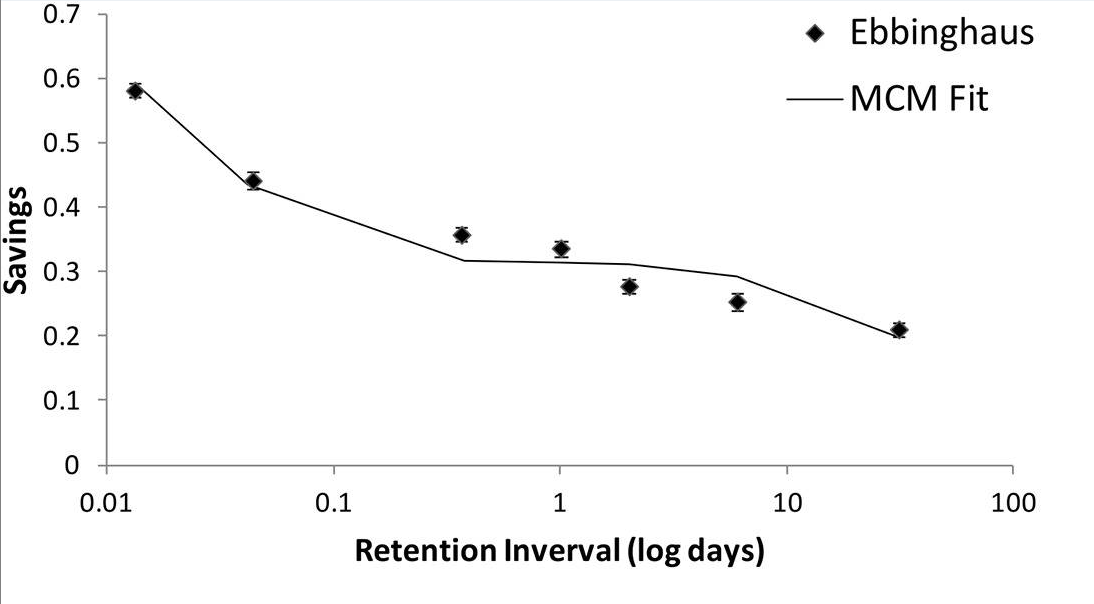
\includegraphics[width=0.60\textwidth]{figures/ebbinghaus_curve.png}
            \caption{The forgetting curve, with original data from Ebbinghaus \cite{ebbinghaus1885memory}, as replotted by Murre and Dros \cite{murre2015replication}. Image: Jaap M. J. Murre, Wikimedia Commons, CC BY 4.0.}
            \label{fig:ebbinghaus_curve}
        \end{figure}

        \subsubsection{Classic Leitner's Algorithm}
        \label{subsubsec:leitner}
        The Leitner system operationalised the forgetting curve as a simple, non-parametric scheduling heuristic decades before it became computationally tractable to fit an individual decay curve per item \cite{leitner1972lernen}. Flashcards are sorted into a series of boxes; a card answered correctly is promoted one box forward, to be reviewed at a longer interval, while a card answered incorrectly is reset all the way back to the first box, regardless of how far it had previously advanced, to be reviewed again at the shortest interval. The scheme requires no numerical memory model at all --- the box number is a coarse, discretised proxy for the item's memory strength $S$ --- which makes it trivially implementable but insensitive to the fact that different items, and different learners, decay at markedly different rates even within the same box.

        \begin{figure}[!htbp]
            \centering
            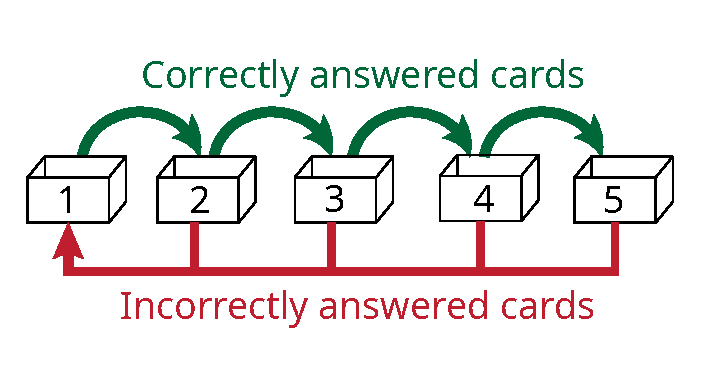
\includegraphics[width=0.62\textwidth]{figures/leitner_system.pdf}
            \caption{The classic five-box Leitner scheduling system. Image: Zirguezi, Wikimedia Commons \cite{zirguezi2012leitner}, CC0 1.0.}
            \label{fig:leitner_system}
        \end{figure}

        \subsubsection{Parametric Half-Life Regression}
        \label{subsubsec:hlr}
        Duolingo's half-life regression (HLR) model, introduced in 2016 \cite{settles2016trainable}, replaces the Leitner system's discrete boxes with a continuous, per-item, per-learner estimate of the memory half-life $h$ --- the elapsed time at which recall probability has decayed to 50\%. Recall probability $p$ for a given item is modelled as an exponential decay in the elapsed interval $\Delta t$ since it was last reviewed, directly generalising the Ebbinghaus curve of Section~\ref{subsubsec:ebbinghaus}:
        \begin{equation}
            \label{eq:hlr_recall}
            p = 2^{-\Delta t / h}
        \end{equation}
        The half-life $h$ itself is not fixed but estimated per item and per learner via a log-linear regression over a feature vector $\mathbf{x}$ --- such as the number of prior correct and incorrect attempts --- with a learned weight vector $\boldsymbol{\Theta}$:
        \begin{equation}
            \label{eq:hlr_halflife}
            \hat{h}_{\boldsymbol{\Theta}}(\mathbf{x}) = 2^{\boldsymbol{\Theta} \cdot \mathbf{x}}
        \end{equation}
        generalising the Leitner box index into a continuously-valued, learner- and item-specific quantity. The weight vector $\boldsymbol{\Theta}$ is not known in advance: it must itself be fitted offline, by regression over a large historical corpus of review outcomes pooled across many users, before Equation~\ref{eq:hlr_halflife} can be applied to a single new one --- Settles and Meeder trained their original model on Duolingo's own multi-million-user interaction log \cite{settles2016trainable}. A newly-launched application, without an equivalent corpus of prior review data from which to fit $\boldsymbol{\Theta}$, cannot reproduce this regression from its own history alone. Section~\ref{subsubsec:fsrs} reviews an alternative memory model that avoids this cold-start requirement.

        \subsubsection{FSRS and the DHP Model}
        \label{subsubsec:fsrs}
        The Free Spaced Repetition Scheduler (FSRS) originates in the DHP model developed at MaiMemo \cite{ye2022stochastic}, a variant of what the open-source scheduling community terms the \textbf{DSR} model: memory state is represented not by a single half-life $h$, as in HLR, but by three jointly-updated variables --- \textbf{difficulty} $D \in [1, 10]$ (how intrinsically hard the item is to learn), \textbf{stability} $S$ (the number of days for retrievability to decay to 90\%), and \textbf{retrievability} $R$ (the instantaneous, momentary probability of successful recall, analogous to $p$ in HLR). Each is revised after every individual review rather than re-estimated from scratch, and each review is scored on a four-point grade $G \in \{1,2,3,4\}$ (\emph{again}, \emph{hard}, \emph{good}, \emph{easy}). Since its first release, FSRS has been refined through several major versions (v1 through the current FSRS-6), each adding parameters and improving the empirical fit of its forgetting curve and update rules \cite{opensr2026algorithm}; the formulation below is the current one (FSRS-6), noting where it revises earlier versions.

        \paragraph{The forgetting curve.} Rather than the fixed exponential decay of Equation~\ref{eq:hlr_recall}, FSRS models retrievability as a power-law function of the elapsed interval $t$ and the current stability $S$, with a trainable decay exponent $w_{20}$ (the $w_i$ denote the elements, $0$-indexed, of a fitted 21-parameter weight vector $\mathbf{w}$):
        \begin{equation}
            \label{eq:fsrs_retrievability}
            R(t, S) = \left(1 + \text{factor} \cdot \frac{t}{S}\right)^{-w_{20}}, \qquad \text{factor} = 0.9^{-1/w_{20}} - 1,
        \end{equation}
        where the factor term is chosen precisely so that $R(S, S) = 0.9$ always holds, preserving stability's definition regardless of the fitted value of $w_{20}$. This is itself the product of two earlier simplifications: the original FSRS v4 fixed the exponent at $w_{20}=1$ with $\text{factor}=1/9$, reducing Equation~\ref{eq:fsrs_retrievability} to $R(t,S) = (1 + t/9S)^{-1}$; FSRS-4.5 refined this to a fixed exponent of $0.5$; only from FSRS-5 onward is the decay shape itself learned from data.

        \paragraph{Initial state and difficulty updates.} A word's very first review initialises stability and difficulty directly from the grade it receives:
        \begin{equation}
            \label{eq:fsrs_initial}
            S_0(G) = w_{G-1}, \qquad D_0(G) = w_4 - e^{w_5 (G-1)} + 1,
        \end{equation}
        so that, for instance, an item first rated \emph{again} ($G=1$) starts at the lowest stability $w_0$ and the highest difficulty $D_0(1) = w_4$. On every subsequent review, difficulty drifts by a grade-dependent increment and is then pulled back towards a fixed target via \emph{mean reversion}:
        \begin{equation}
            \label{eq:fsrs_difficulty}
            D' = D - w_6 (G - 3) \cdot \frac{10 - D}{9}, \qquad D'' = w_7 \, D_0(4) + (1 - w_7) \, D',
        \end{equation}
        anchoring difficulty to $D_0(4)$ (the initial difficulty of an \emph{easy}-rated item) rather than letting it drift unboundedly after a long run of easy or hard grades --- informally termed avoiding ``ease hell'' in the flashcard-scheduling community.

        \paragraph{Stability updates.} Following a successful review ($G \in \{2,3,4\}$), stability increases according to
        \begin{equation}
            \label{eq:fsrs_stability_recall}
            S_r'(D, S, R, G) = S \cdot \Big(e^{\,w_8 (11 - D) \, S^{-w_9} \left(e^{w_{10}(1-R)} - 1\right) \cdot w_{15}^{[G=2]} \cdot w_{16}^{[G=4]}} + 1\Big),
        \end{equation}
        while a lapse ($G=1$) instead resets stability to a smaller post-lapse value,
        \begin{equation}
            \label{eq:fsrs_stability_forget}
            S_f'(D, S, R) = w_{11} \, D^{-w_{12}} \left((S+1)^{w_{13}} - 1\right) e^{w_{14}(1-R)}.
        \end{equation}
        Writing $S_{\mathrm{inc}} = S_r'/S$ for the multiplicative stability gain of a successful review, three qualitative properties of Equation~\ref{eq:fsrs_stability_recall} recur throughout the FSRS documentation and are directly interpretable in terms of the theory already established in this chapter: $S_{\mathrm{inc}}$ decreases as difficulty $D$ increases (harder items consolidate more slowly); $S_{\mathrm{inc}}$ decreases as stability $S$ itself increases (an already well-consolidated memory is harder to strengthen further, consistent with the diminishing-returns shape of the Ebbinghaus curve in Section~\ref{subsubsec:ebbinghaus}); and $S_{\mathrm{inc}}$ increases as retrievability $R$ decreases at the time of review, i.e.\ a successful recall of an \emph{almost-forgotten} item strengthens memory more than reviewing an item that was never at risk --- the computational signature of the spacing effect.

        \paragraph{Same-day reviews (FSRS-6).} The formulas above govern reviews spaced at least a day apart. FSRS-6's specific contribution is a separate, more conservative update for a card reviewed again on the same day it was last seen:
        \begin{equation}
            \label{eq:fsrs_stability_sameday}
            S'(S, G) = S \cdot e^{\,w_{17}(G - 3 + w_{18}) \, S^{-w_{19}}},
        \end{equation}
        which grows quickly while $S$ is still small and flattens as $S$ grows, converging once $S_{\mathrm{inc}} = e^{w_{17}(G-3+w_{18})S^{-w_{19}}} = 1$; earlier versions used the same functional form without the $S^{-w_{19}}$ damping term, allowing same-day repetition to inflate stability unrealistically.

        This finer-grained decomposition is, at the time of writing, the most empirically accurate publicly documented model of spaced-repetition scheduling. Critically for a new application, all of Equations~\ref{eq:fsrs_retrievability}--\ref{eq:fsrs_stability_sameday} update the per-item state \emph{incrementally, after each individual review}, using a fixed parametric rule rather than a regression re-fitted in a single offline pass over a large historical corpus, as HLR requires (Section~\ref{subsubsec:hlr}). A new item begins from the initial-state Equation~\ref{eq:fsrs_initial} and refines its own difficulty and stability purely from the learner's own subsequent review history, without needing Duolingo-scale historical data first; \textit{Glosy} adopts the published default parameter vector $\mathbf{w}$ rather than fitting its own, precisely because it does not yet have the review corpus such a fit would require. This is the specific reason Chapter~\ref{methodology}, Section~\ref{sec:recommendation} (Stage 2) adopts the FSRS formulation, rather than HLR, as the basis of the \texttt{SRS\_Urgency} scoring term in the recommendation engine: a word's recommendation urgency rises as its predicted retrievability $R$ (Equation~\ref{eq:fsrs_retrievability}) falls.

    \subsection{Active Recall and the Testing Effect}
    \label{subsec:testing_effect}
    A separate, complementary strand of cognitive psychology addresses not \emph{when} to review an item, but \emph{how}. The testing effect --- robustly demonstrated across decades of memory research --- shows that the act of actively retrieving an item from memory (as in a test or a recall task) produces substantially better long-term retention than an equivalent amount of time spent passively re-studying the same item \cite{roediger2006testing}. This finding motivates a specific design constraint distinct from, and additional to, the scheduling question addressed by Section~\ref{subsec:srs_models}: \emph{when} an item is due for review, the review task itself should require productive retrieval (e.g., recalling and typing a word) rather than passive recognition (e.g., selecting a familiar-looking option among distractors). Section~\ref{subsec:serious_games} reviews game mechanics through this lens.


% ==============================================================================
% SECTION 3: MODALITIES FOR ACQUISITION AND ACTIVE REINFORCEMENT
% ==============================================================================
\section{Modalities for Language Acquisition}
\label{sec:modalities}

    Sections~\ref{subsec:comprehensible_input}--\ref{subsec:testing_effect} establish \emph{what} an effective input and reinforcement episode should look like theoretically: comprehensible ($i+1$), authentic, cognitively bounded, spaced, and actively recalled. This section reviews the empirical literature on the two content modalities through which \textit{Glosy} delivers input and reinforcement respectively: short-form video, addressed to the input side of acquisition, and serious games, addressed to the active-recall side.

    \subsection{Short-Form Video in Second Language Acquisition (SLA)}
    \label{section:reels_in_sla}

        \subsubsection{Incidental Vocabulary Acquisition through Audiovisual Input}
        A substantial body of research in Computer-Assisted Language Learning (CALL) predates the short-form video format itself and concerns the closely related case of captioned television and film viewing. Vanderplank's early work on teletext subtitles found that captioned video supports vocabulary and listening development beyond what audio alone provides, by allowing the learner to cross-reference the written and spoken forms of an unfamiliar item in real time \cite{vanderplank1988value}. More recent corpus-informed work confirms this incidental-learning effect at scale: Peters and Webb found measurable incidental vocabulary gains from watching L2 television programmes without any explicit study task, with gains moderated by frequency of item occurrence and by the presence of captions \cite{peters2018incidental}, while Montero Perez, Peters, and Desmet found that enhancing target vocabulary within video captions (e.g., through highlighting) further improves retention relative to unenhanced captioned video \cite{monteroperez2018vocabulary}. Taken together, this literature establishes that passive audiovisual viewing is a genuine, if modest, channel of incidental vocabulary acquisition, and that the effect is strengthened, not weakened, by textual scaffolding synchronised to the audio track --- precisely the token-level, timestamped transcript structure that a \textit{Glosy} reel provides (Chapter~\ref{methodology}, Section~\ref{sec:data_modelling}).

        \subsubsection{The Gap: Passive Consumption without Reinforcement}
        \label{subsubsec:passive_consumption_gap}
        The incidental-acquisition literature reviewed above is consistent in one further respect: the vocabulary gains it reports from passive viewing alone are real but small, typically requiring many repeated incidental encounters of an item before it is durably retained \cite{peters2018incidental}. Passive viewing, in other words, is an effective delivery mechanism for comprehensible input (Section~\ref{subsec:comprehensible_input}) but is not, by itself, a spaced-repetition system in the sense of Section~\ref{subsec:srs_models}: a viewer has no mechanism by which an encountered item is tracked, scheduled for review, or actively retrieved once the video ends. This is the specific gap in generic short-form social video consumption --- as opposed to a purpose-built application --- that motivates the research question posed in Chapter~\ref{chapter:intro}: watching unstructured reels on an existing social platform provides input without a tracked vocabulary state, and therefore without the scheduled, active-recall reinforcement that Sections~\ref{subsec:srs_models} and~\ref{subsec:testing_effect} identify as necessary for durable retention. Closing this gap requires attaching a conventional SRS review step --- of the kind ordinarily triggered by a static flashcard in an application such as Anki --- directly to the moment a due item is encountered inside a reel, rather than leaving that encounter to pass by unrecorded. Chapter~\ref{methodology} details the interface through which \textit{Glosy} does this: a due word appearing in a reel's transcript prompts an in-context review step immediately after viewing, through which the learner's recall grade $G$ is captured and fed into the FSRS update rules of Section~\ref{subsubsec:fsrs} (Equations~\ref{eq:fsrs_stability_recall}--\ref{eq:fsrs_stability_forget}) --- the reel itself standing in for the static flashcard as the review's triggering stimulus.

    \subsection{Serious Games and Gamification in Language Learning}
    \label{subsec:serious_games}

        \subsubsection{Game-Based Learning versus Gamification}
        \label{subsubsec:gbl_vs_gamification}
        Section~\ref{subsec:platform_limitations} (item 4) distinguished \emph{gamification} --- decorating an existing task with game-design elements such as points and streaks \cite{deterding2011gamification} --- from \emph{game-based learning}, in which the instructional content is embedded within the mechanical loop of an actual game \cite{plass2015foundations}. This distinction is well established as a specific research strand within CALL: Godwin-Jones's review of games in language learning documents a persistent gap between the two, noting that commercially successful language-learning products have historically favoured drill-based gamification because it is comparatively cheap to build and easy to monetise, while games in which linguistic competence is itself the win condition remain comparatively rare \cite{godwinjones2014games}. Sykes and Reinhardt's broader treatment of digital games in second and foreign language teaching similarly argues that a game's pedagogical value derives from whether target-language production or comprehension is load-bearing to \emph{winning the game}, not merely rewarded upon completion of an unrelated exercise \cite{sykes2013language}.

        \subsubsection{Difficulty Adaptation in Hypercasual Games}
        \label{subsubsec:dda}
        Section~\ref{sub:hypercasual_and_hybrid_casual_games} (Chapter~\ref{chapter:intro}) established the hypercasual genre's core appeal: minimal onboarding, immediately intuitive mechanics, and short session length --- properties that align closely with the microlearning argument of Section~\ref{subsec:cognitive_load_microlearning}. Within game design more specifically, dynamic difficulty adjustment (DDA) --- algorithmically tuning a hypercasual game's difficulty in response to the individual player's observed performance, rather than fixing it in advance --- has been shown to improve player retention and perceived replay value relative to a static difficulty curve \cite{yang2020hyper}. This provides the game-design-theoretic counterpart to the lexical personalisation argument of Section~\ref{sec:recommendation_algorithms}: just as a reel should be selected for lexical comprehensibility, a game level's difficulty should be tuned to the player's demonstrated skill --- in \textit{Glosy}'s case, the specific vocabulary items the level is built from, rather than a generic difficulty parameter.

        \subsubsection{Active-Recall Game Mechanics for Vocabulary}
        \label{subsubsec:active_recall_games}
        The testing-effect literature reviewed in Section~\ref{subsec:testing_effect} \cite{roediger2006testing} favours game mechanics that require \emph{productive} retrieval of a target word's orthographic form over mechanics that require only its \emph{recognition} among distractors. Word-reconstruction puzzle formats --- in which the player must recall and produce a target word letter-by-letter, validating each attempt against positional or compositional constraints --- structurally enforce this kind of active retrieval as the core win condition of the game itself, rather than as an optional or bypassable step. This is the specific theoretical property, rather than genre popularity alone, that motivates the word-reconstruction game modalities implemented in \textit{Glosy} and documented in Chapter~\ref{methodology}, Section~\ref{sec:games_design}.


% ==============================================================================
% SECTION 4: ALGORITHMIC FRAMEWORKS FOR PERSONALIZED RECOMMENDATION
% ==============================================================================
\section{Algorithmic Frameworks for Personalized Recommendation}
\label{sec:recommendation_algorithms}

    Sections~\ref{sec:pedagogical_foundations} and~\ref{sec:modalities} establish \emph{which} content is pedagogically appropriate for a learner at a given moment: comprehensible (Section~\ref{subsec:comprehensible_input}), due for review (Section~\ref{subsec:srs_models}), and appropriately reinforcing (Section~\ref{sec:modalities}). Selecting such content automatically, per learner, is a recommendation problem in the information-retrieval sense. This section reviews the two classical recommendation paradigms, content-based and collaborative filtering, and the strategies the literature offers for combining them; Section~\ref{sec:synthesis} maps this theory onto \textit{Glosy}'s own recommendation engine.

    \subsection{Content-Based Filtering}
    \label{subsec:content_based_filtering}
    Content-based filtering recommends items by comparing an item's own features against a profile of a single user's own preferences, built from that user's history, without reference to other users' behaviour \cite{adomavicius2005toward}. Its principal known limitation is that it has no way to express a temporal signal such as \emph{when} a previously-seen item is due for review \cite{adomavicius2005toward} --- a gap the memory-decay models of Section~\ref{subsec:srs_models} are specifically designed to fill.

    \subsection{Collaborative Filtering and Hybrid Recommender Systems}
    \label{subsec:cascade_hybrid}
    Collaborative filtering (CF) recommends items based on patterns of agreement across many users' behaviour --- favouring items that users with a similar engagement history have responded well to --- rather than on an item's own features \cite{adomavicius2005toward}. Because it depends on an interaction matrix populated across many users, CF is known to perform poorly under the \emph{cold-start} problem, when a system has few users or little accumulated interaction history \cite{adomavicius2005toward}.

    Burke's survey of hybridisation strategies for combining multiple recommendation techniques distinguishes several ways of doing so, including \emph{weighted} hybridisation, in which each technique produces an independent score and the final score is their linear combination, and \emph{cascade} hybridisation, in which one technique coarsely ranks or partitions the candidate set and a second technique is applied only to break ties within it \cite{burke2002hybrid}. Ricci et al.'s handbook situates both strategies, and content-based and collaborative filtering more generally, within the broader design space of recommender systems \cite{ricci2011introduction}.

    \subsection{Recommender Systems in Educational Technology}
    \label{subsec:edtech_recommenders}
    Recommender systems applied to e-learning typically personalise the sequencing of resources or exercise \emph{difficulty} to a learner's inferred ability, rather than the semantic content of what is recommended \cite{klasnja2011elearning} --- the same gap identified in Section~\ref{subsec:platform_limitations} (item~1).


% ==============================================================================
% SECTION 5: SYNTHESIS -- A THEORY-DRIVEN DESIGN FRAMEWORK
% ==============================================================================
\section{Synthesis: A Theory-Driven Design Framework}
\label{sec:synthesis}

    This chapter has reviewed, in turn, the pedagogical theory of comprehension and retention (Section~\ref{sec:pedagogical_foundations}), the empirical literature on the two content modalities through which \textit{Glosy} delivers input and reinforcement (Section~\ref{sec:modalities}), and the algorithmic frameworks by which content is selected and sequenced for the individual learner (Section~\ref{sec:recommendation_algorithms}). Table~\ref{tab:theory_synthesis} makes explicit the traceability between each theoretical foundation reviewed above and the corresponding design decision it motivates in Chapter~\ref{methodology}, operationalising the theory-driven design approach stated at the outset of Section~\ref{sec:pedagogical_foundations}.

    \begin{table}[htbp]
        \centering
        \small
        \caption{Theory-driven design traceability matrix: theoretical foundation, design implication, and the corresponding Glosy component.}
        \label{tab:theory_synthesis}
        \begin{tabular}{p{3.6cm}p{4.6cm}p{4.6cm}}
            \hline
            \textbf{Theoretical Foundation} & \textbf{Design Implication} & \textbf{Glosy Component} \\
            \hline
            ZPD (\ref{subsec:sociocultural_theory}) \& Input Hypothesis (\ref{subsec:comprehensible_input}) &
            Recommend content at the $i+1$ comprehensibility boundary &
            Stage 1: Comprehensibility Filtering, 98\% lexical coverage (Sec.~\ref{subsec:stage1_design}) \\
            \hline
            Cognitive Load Theory \& Microlearning (\ref{subsec:cognitive_load_microlearning}) &
            Bound each learning episode to a short, self-contained unit &
            90-second reel cap; Wordle attempt limit; Word of Wonders word/letter caps (Sec.~\ref{sec:system_overview}, Sec.~\ref{sec:games_design}) \\
            \hline
            Forgetting Curve \& Spaced Repetition (\ref{subsec:srs_models}) &
            Schedule review before predicted recall failure &
            Stage 2: Spaced-Repetition Prioritisation, due-word partitioning (Sec.~\ref{subsec:stage2_design}) \\
            \hline
            Testing Effect (\ref{subsec:testing_effect}) \&
            Game-Based Learning (\ref{subsec:serious_games}) &
            Require productive retrieval, not passive recognition &
            Wordle-style and Word of Wonders vocabulary games (Sec.~\ref{sec:games_design}) \\
            \hline
            Cascade Hybrid Recommender (\ref{subsec:cascade_hybrid}) &
            Filter by comprehensibility, partition by due-for-review, break ties by engagement-weighted content similarity &
            Stage 1--3 cascade ranking (Sec.~\ref{subsec:cascade_design}) \\
            \hline
            Sociocultural Theory (\ref{subsec:sociocultural_theory}) &
            Provide social scaffolding for culturally-opaque authentic input &
            Collaborative learning features (Ch.~\ref{chapter:conclusions}, Future Work) \\
            \hline
        \end{tabular}
    \end{table}

    Read together with the platform limitations identified in Section~\ref{subsec:platform_limitations}, this synthesis reframes the research questions posed in Chapter~\ref{chapter:intro} as a design problem with a specific theoretical answer for each of its parts: RQ1 is addressed by the content-based lexical filtering of Section~\ref{subsec:content_based_filtering} operating over the short-form video modality of Section~\ref{section:reels_in_sla}; RQ2 is addressed by the cascade hybrid of Section~\ref{subsec:cascade_hybrid}, fusing comprehensibility with the memory-decay models of Section~\ref{subsec:srs_models}; and RQ3 is addressed by the active-recall game theory of Section~\ref{subsec:serious_games}, parameterised by the same memory-decay state that governs RQ2. Chapter~\ref{methodology} now presents the system architecture that implements this framework.

\newpage


\chapter{System Architecture \& Methodology} \label{methodology}
\section{System Overview}


    \begin{itemize}
        \item \textbf{Frontend:}
        \item \textbf{Backend API:}
        \item \textbf{Reels Service:}
        \item \textbf{Database:}
    \end{itemize}

    \begin{figure}[htbp]
        \centering
        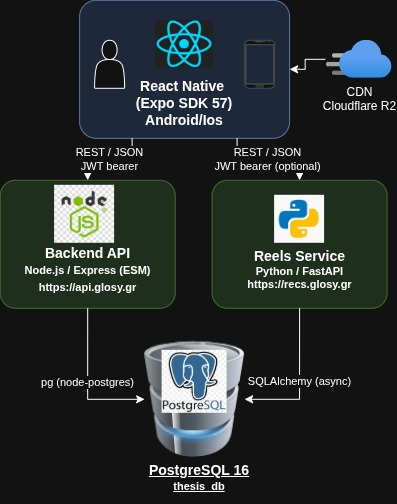
\includegraphics[width=0.85\textwidth]{figures/architecture.pdf}
        \caption{High-level system architecture: the mobile frontend communicates with the Backend API (\texttt{api.glosy.gr}) and the Reels Service (\texttt{recs.glosy.gr}) over authenticated REST endpoints; both services share a single PostgreSQL instance.}
        \label{fig:architecture}
    \end{figure}


\section{Technology Stack}
\label{sec:tech_stack}
    \subsection{Frontend --- React Native / Expo}
    \label{subsec:frontend_stack}

    \subsection{Backend API --- Node.js / Express}
    \label{subsec:backend_stack}

    \subsection{Reels Service --- Python / FastAPI}
    \label{subsec:reels_stack}

    \subsection{Database --- PostgreSQL}
    \label{subsec:db_stack}


\section{Data Modelling} \label{sec:data_modelling}
    \subsection{Linguistic Content}
    \label{subsec:data_linguistic}

    \subsection{User State}
    \label{subsec:data_user_state}

    \subsection{Engagement Signals}
    \label{subsec:data_engagement}


\section{Recommendation Engine Design} \label{sec:recommendation}
    \subsection{Stage 1: Comprehensibility Filtering}
    \label{subsec:stage1_design}

        \begin{equation}
            \text{Coverage}(U, R) = \frac{|V_R \cap V_U|}{|V_R|} \ge 0.98
        \end{equation}
        where $V_R$ is the unique set of lexical tokens in reel $R$, and $V_U$ represents the known vocabulary lexicon of user $U$.

    \subsection{Stage 2: Spaced-Repetition Prioritisation}
    \label{subsec:stage2_design}

    \subsection{Stage 3: Content-Based Personalisation}
    \label{subsec:stage3_design}

    \subsection{Combining the Three Stages: A Cascade, Not a Weighted Sum}
    \label{subsec:cascade_design}


\section{Gamification Design}
\label{sec:gamification_design}
    \subsection{Progression Currencies: Coins, Energy, and Experience}
    \label{subsec:currencies_design}

    \subsection{Design Principle: Every Game Round Doubles as an FSRS Review}
    \label{subsec:game_review_design}


\section{Vocabulary-Driven Games}
\label{sec:games_design}
    \subsection{Wordle-Style Game}
    \label{subsec:wordle_design}

    \subsection{Word of Wonders (Crossword)}
    \label{subsec:wow_design}


\newpage


\chapter{Implementation Details} \label{chapter:discussion}
\section{Database Schema}
\label{sec:db_schema}
    \subsection{Linguistic Content Tables}
    \label{subsec:schema_linguistic}

    \subsection{User State Tables}
    \label{subsec:schema_user_state}

    \subsection{Engagement Signal Tables}
    \label{subsec:schema_engagement}


\section{Backend API}
\label{sec:backend_api}
    The API has been documented using Swagger/OpenAPI. The documentation is available at \texttt{/swagger} endpoint.

    \subsection{Authentication and Authorization}
    \label{subsec:auth_impl}
        \subsubsection{JWT Access/Refresh Token Rotation}
        \subsubsection{Google OAuth 2.0}

    \subsection{Registration and Vocabulary Initialisation}
    \label{subsec:registration_impl}
        \subsubsection{Proficiency-Based Vocabulary Auto-Seeding}

    \subsection{Offline Synchronisation}
    \label{subsec:sync_impl}
        \subsubsection{Change-Set Ordering: Deletes, Updates, Inserts}

    \subsection{Dictionary and Letters Modules}
    \label{subsec:dictionary_impl}


\section{Frontend Architecture}
\label{sec:frontend_arch}
    \subsection{Navigation and Screen Structure}
    \label{subsec:navigation_impl}

    \subsection{State Management: Context and Hooks}
    \label{subsec:state_mgmt_impl}

    \subsection{Offline-First Strategy}
    \label{subsec:offline_impl}


\section{Reels Service}
\label{sec:reels_service_impl}
    \subsection{Service Architecture}
    \label{subsec:reels_arch_impl}
    The reels microservice (\texttt{reels-service/}) is a FastAPI python application.

    \subsection{Reel Creation and Dialogue Enrichment}
    \label{subsec:reel_creation_impl}
    Each uploaded reel response embeds the full dialogue associated with the reel's video content.

    \subsection{Recommendation Engine Implementation}
    \label{subsec:recommendation_impl}
        \subsubsection{Stage 1: SQL-Level Comprehensibility Filtering}
        \subsubsection{Stage 2: Frontend-Supplied Due-Word Partitioning}
        \subsubsection{Stage 3: TF-IDF Profile Vectors and Cosine Similarity}

    \subsection{Personalisation Implementation Status}
    \label{subsec:personalisation_status}


\section{Game Modules}
\label{sec:game_modules_impl}
    \subsection{Wordle-Style Game Implementation}
    \label{subsec:wordle_impl}

    \subsection{Word of Wonders: Procedural Crossword Generation}
    \label{subsec:wow_impl}
        \subsubsection{Word Placement and Intersection Search}
        \subsubsection{Letter-Budget and Word-Priority Heuristics}
        \subsubsection{Due-Word Injection as the Practice Word}


\newpage


\chapter{Evaluation \& Results} \label{chapter:evaluation_results}
\section{Evaluation Approach}
\label{sec:eval_approach}
    As acknowledged in Chapter~\ref{chapter:conclusions}, \textit{Glosy} has not yet been evaluated in a controlled study with human learners. This is the main disadvantage of the present work: none of the results in this chapter can speak to actual vocabulary gain, retention, or engagement, since no learner has yet used the system under observation. In the absence of that evidence, this chapter instead evaluates the system's own algorithmic components directly, against real seeded content, to establish whether each behaves as its design in Chapter~\ref{methodology} intends and where it does not --- a necessary but not sufficient substitute for pedagogical evidence, and one that Chapter~\ref{chapter:conclusions} returns to among its directions for future work. Each section below targets one component in isolation, using the real, unmodified implementation from Chapter~\ref{chapter:discussion} rather than a re-derived model of it.

\section{Component-Level Algorithmic Evaluation}
\label{sec:component_eval}

    \subsection{Word of Wonders: Grid-Generation Benchmark}
    \label{subsec:wow_eval}

    The crossword placement algorithm of Section~\ref{subsec:wow_impl} (Algorithms~\ref{alg:wow_placement} and~\ref{alg:wow_priority}) is bounded by three constants: an $8\times8$ board, a practice-word length of at most 8 letters, a shared letter-budget of 8 distinct-letter slots (\texttt{MAX\_LETTERS\_LENGTH}), and a cap of 12 placed words (\texttt{MAX\_WORDS}). Because the algorithm's behaviour depends on how large and how diverse a candidate word pool it is asked to search, and a learner's tracked vocabulary grows from a handful of words at first use to potentially thousands after months of use, the two questions this evaluation asks are: does the generator remain robust as tracked vocabulary grows, and how do the two quantities that matter to a learner --- how rich the resulting puzzle is, and how long they wait for it --- scale with that growth.

    \subsubsection{Method}
    \label{subsubsec:wow_eval_method}
    A benchmark harness (\texttt{scripts/evaluation/wow\_generator/} in the project repository) imports \texttt{LevelGenerator.js} unmodified and drives it with word pools sampled directly from the seeded per-language dictionaries of Section~\ref{sec:data_modelling} (13,373 English, 13,722 Greek, and 14,315 Farsi entries). For each of the three supported languages and seven simulated tracked-vocabulary sizes (10, 100, 500, 1{,}000, 3{,}000, 6{,}000, and 10{,}000 words --- the last comfortably exceeding what any real learner's tracked vocabulary reaches in practice, to characterise the algorithm's behaviour at the extreme rather than only the typical case), 200 repetitions drew an independent random subset of that size from the full dictionary, selected one of its words uniformly at random as the FSRS-due practice word (mirroring \texttt{GameLoader.js}'s own unfiltered selection --- Section~\ref{subsec:game_review_design}), and called the generator exactly as the application does. This produced 4{,}200 trials in total, recording the words placed, the wall-clock generation time, and whether an exception was raised.

    \subsubsection{Robustness}
    Across all 4{,}200 trials, at every vocabulary size in every language, the generator raised no exception and always returned a non-empty board with its practice word placed. This holds even at the smallest tested vocabulary (10 words), where the candidate pool for intersecting words is thin, and at the largest (10{,}000 words), where the priority sort and intersection search run over a considerably larger candidate pool per call than any real session is likely to present it with.

    \subsubsection{Words Placed}
    \label{subsubsec:wow_eval_words_placed}
    \begin{figure}[htbp]
        \centering
        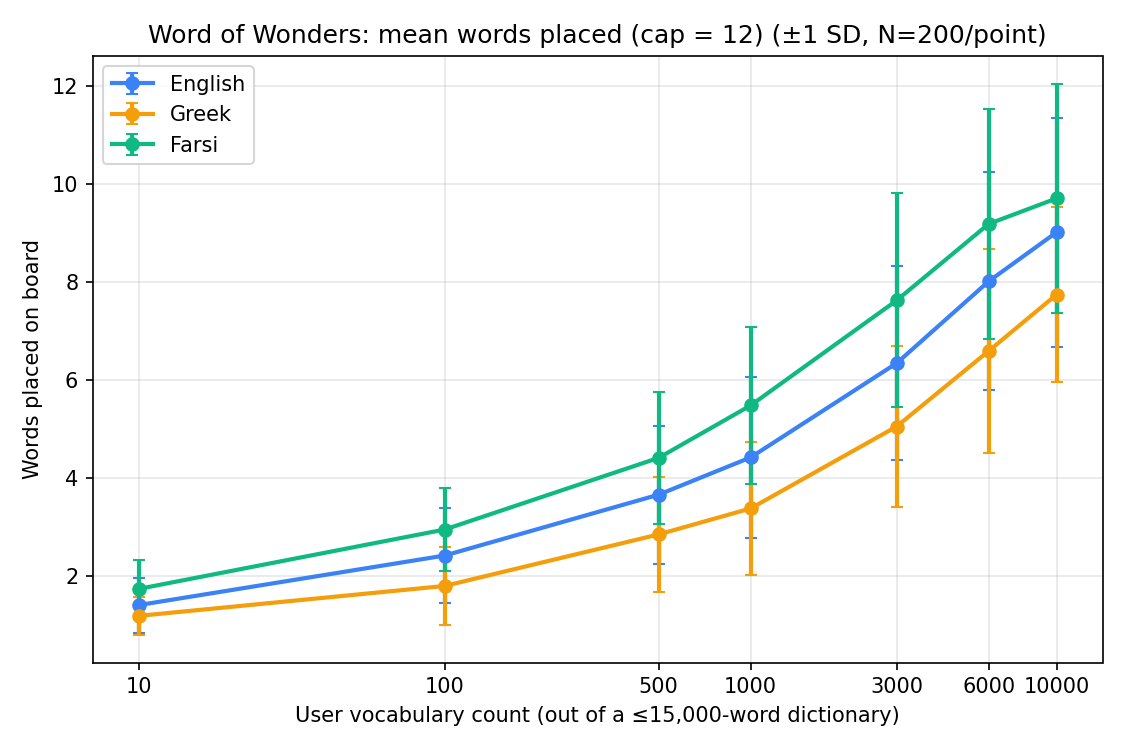
\includegraphics[width=0.8\textwidth]{figures/wow_words_placed.png}
        \caption{Mean words placed on the board (cap = 12) as a function of simulated tracked-vocabulary size, per language. Error bars show $\pm 1$ standard deviation over 200 repetitions per point.}
        \label{fig:wow_words_placed}
    \end{figure}
    Figure~\ref{fig:wow_words_placed} shows words placed rising with vocabulary size in all three languages, from a mean of 1.2--1.8 words at a 10-word vocabulary to 7.7--9.7 words at 10,000 --- yet even at that extreme, the board never saturates the 12-word cap. This confirms the design argument of Section~\ref{subsec:wow_design}: the binding constraint on puzzle richness is the 8-slot letter budget of \texttt{wouldExceedLetterLimit}, not the word count or the cap itself, since a bigger, more diverse candidate pool exhausts the shared letters faster than it exhausts the word cap. A second, consistent pattern across every vocabulary size is a language ordering --- Farsi places the most words, English second, Greek fewest --- consistent with average word length: among the words the generator accepts (three to eight letters after normalisation), the mean length is 5.1 letters for Farsi, 6.0 for English, and 6.5 for Greek, so the language with the shortest words places the most, since a longer average word consumes more of the same 8-letter budget per placement.

    A direct consequence for onboarding is that a brand-new learner, whose tracked vocabulary is by construction small, is served a sparse board of only one or two words rather than a filled one --- compounding, rather than mitigating, the "steep onboarding barriers" limitation already acknowledged in Chapter~\ref{chapter:conclusions}.

    \subsubsection{Qualitative Example: On-Device Boards Across CEFR Levels}
    \label{subsubsec:wow_eval_screenshots}
    \begin{figure}[htbp]
        \centering
        \begin{subfigure}[b]{0.31\textwidth}
            \centering
            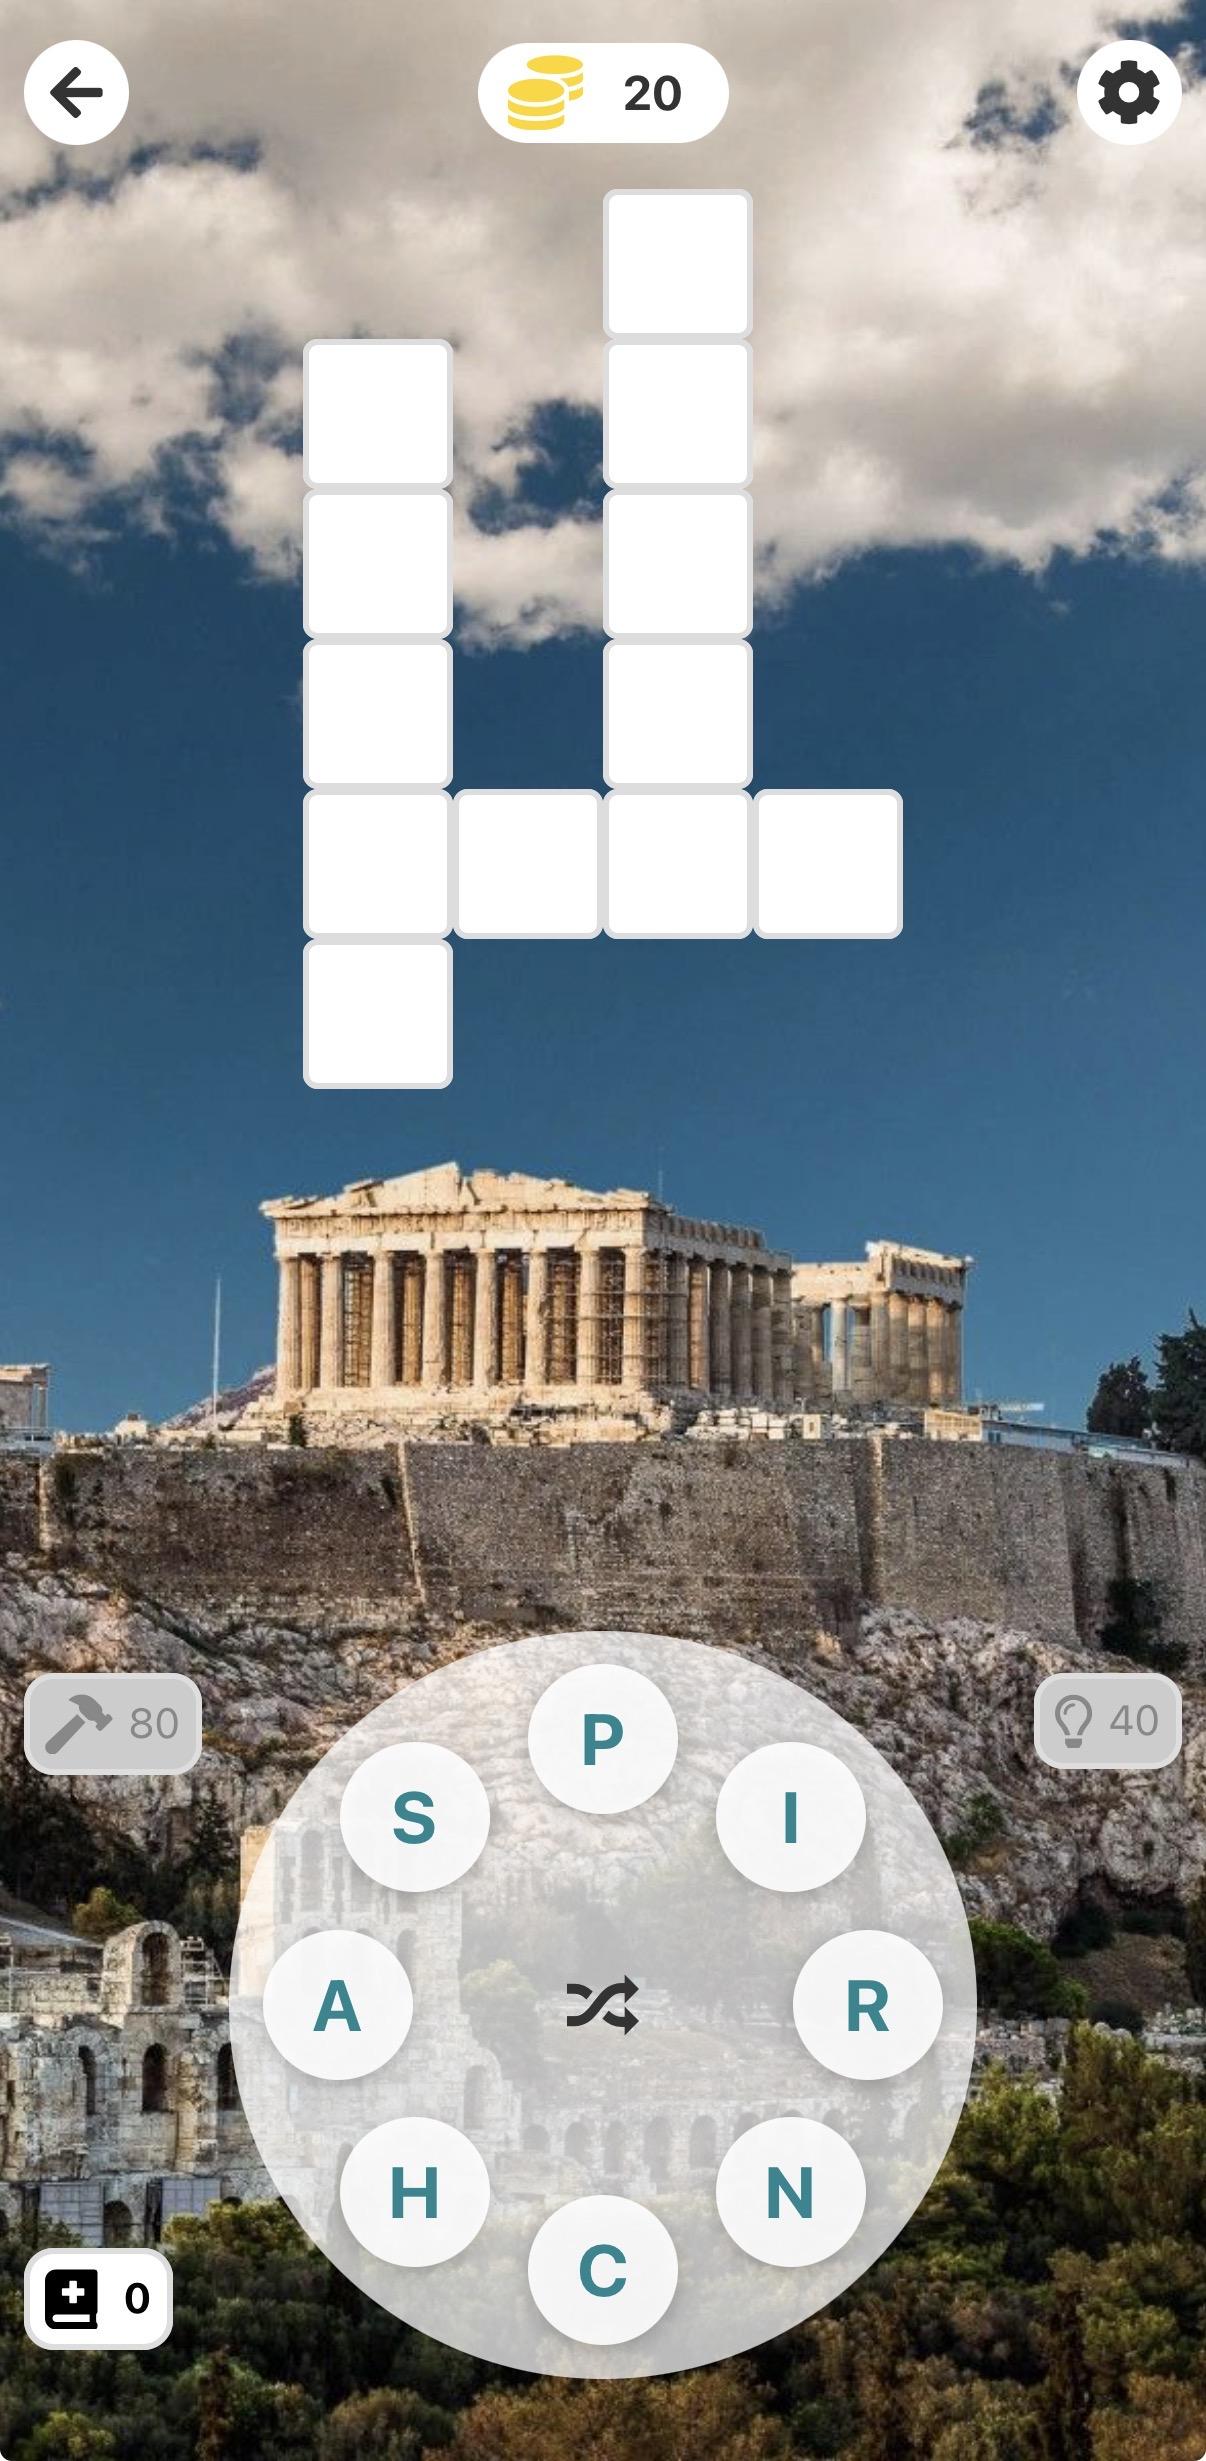
\includegraphics[width=\linewidth]{figures/wow_screenshot_a1.jpg}
            \caption{A1}
            \label{fig:wow_shot_a1}
        \end{subfigure}\hfill
        \begin{subfigure}[b]{0.31\textwidth}
            \centering
            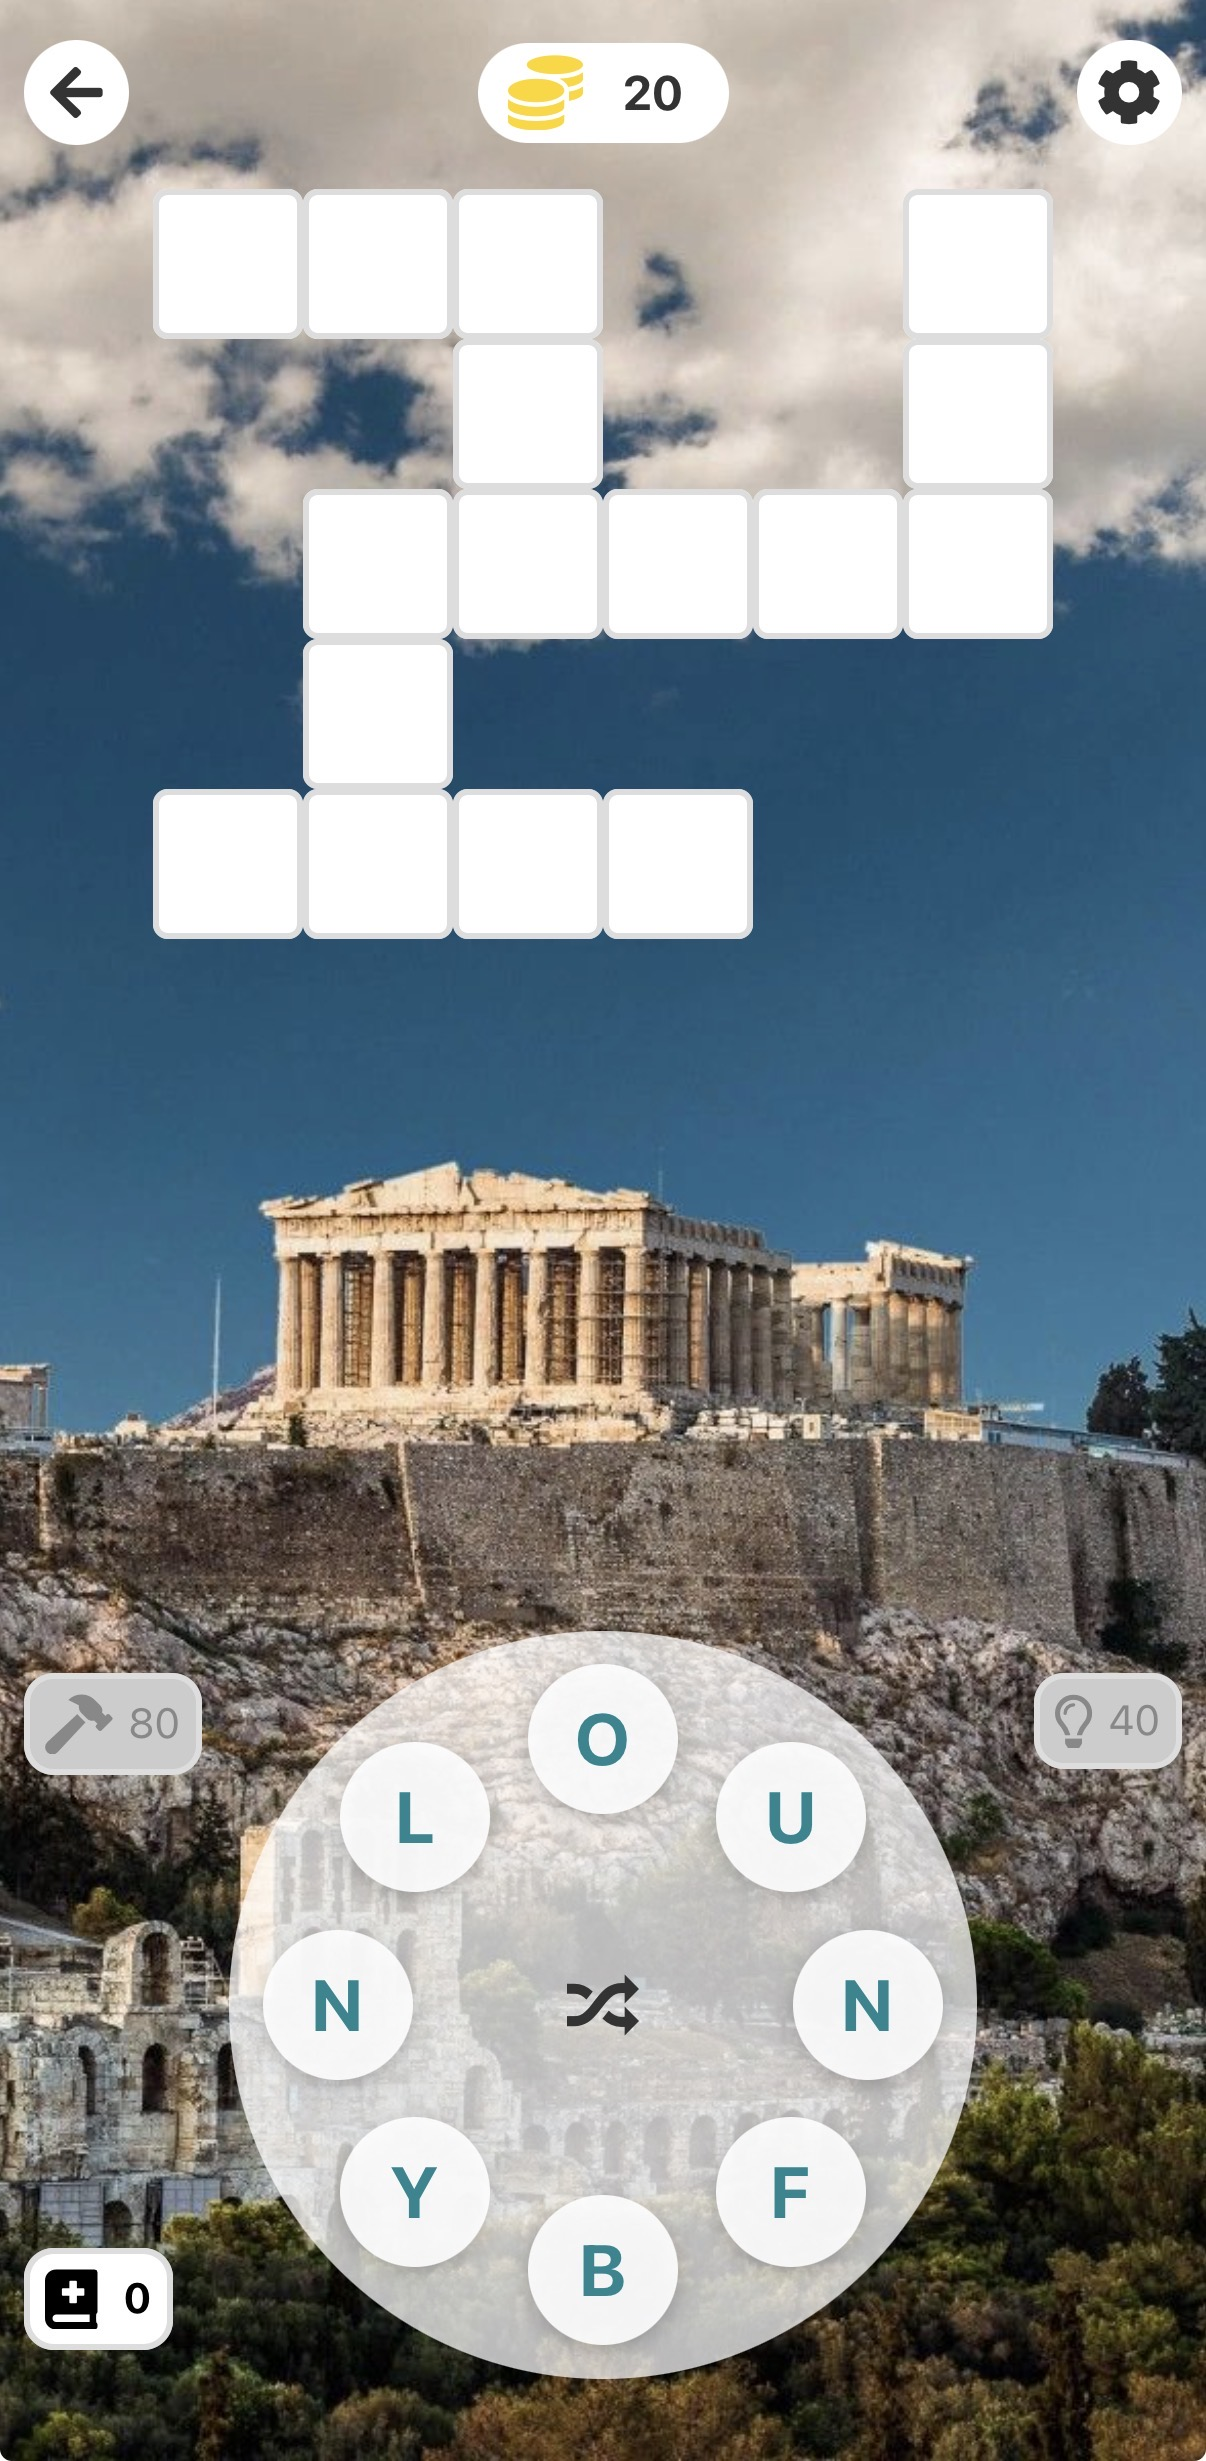
\includegraphics[width=\linewidth]{figures/wow_screenshot_a2.jpg}
            \caption{A2}
            \label{fig:wow_shot_a2}
        \end{subfigure}\hfill
        \begin{subfigure}[b]{0.31\textwidth}
            \centering
            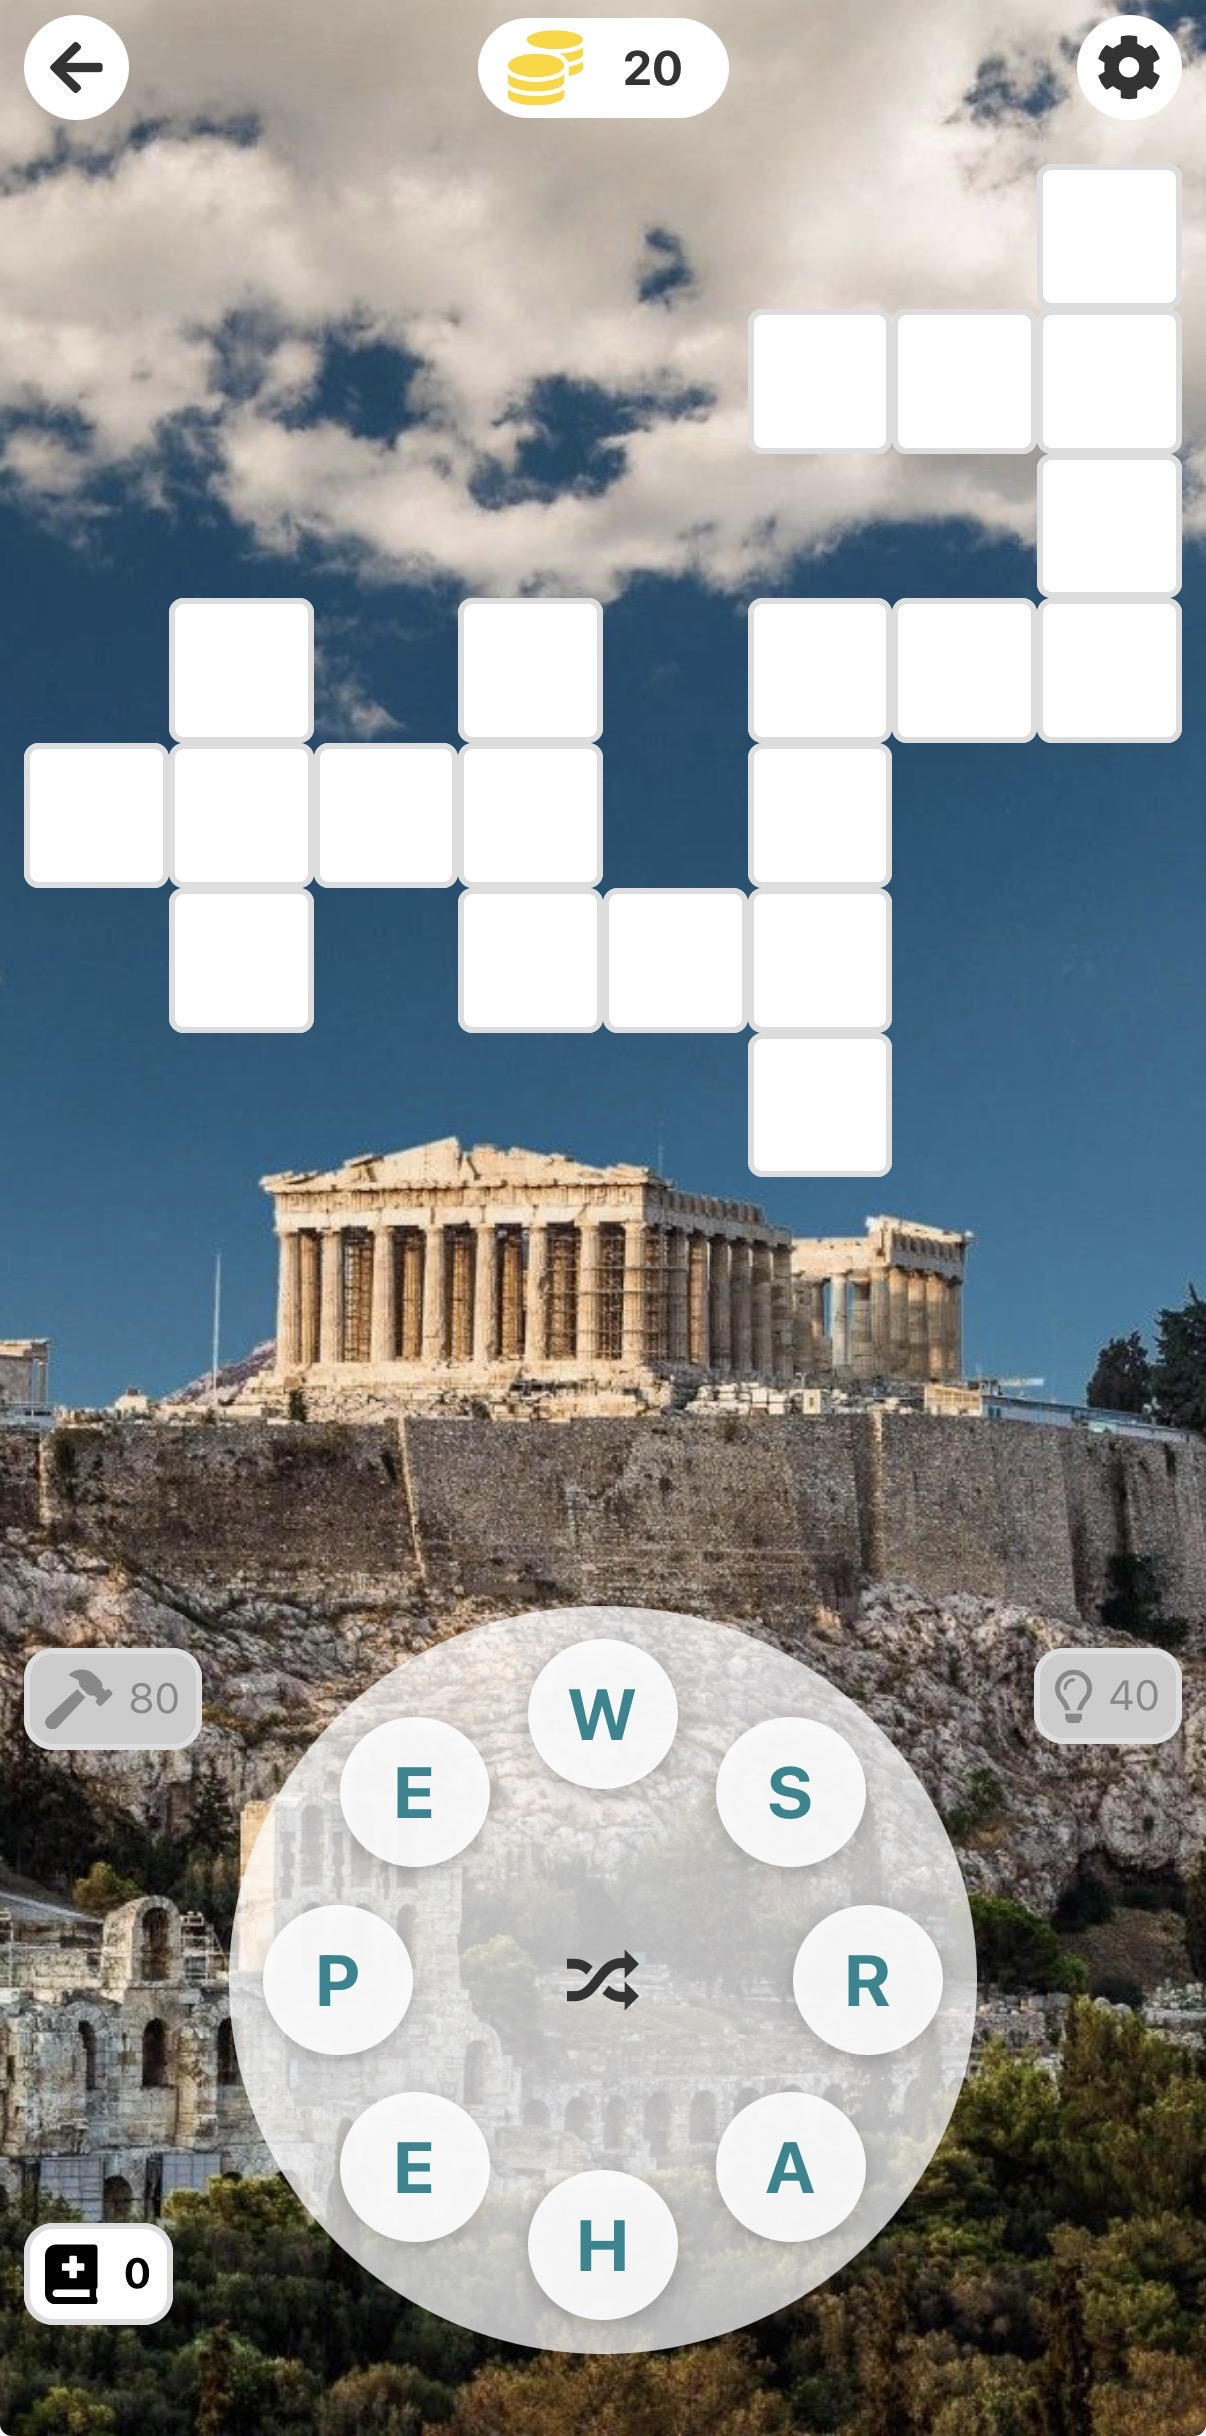
\includegraphics[width=\linewidth]{figures/wow_screenshot_b1.jpg}
            \caption{B1}
            \label{fig:wow_shot_b1}
        \end{subfigure}

        \vspace{1\baselineskip}

        \begin{subfigure}[b]{0.31\textwidth}
            \centering
            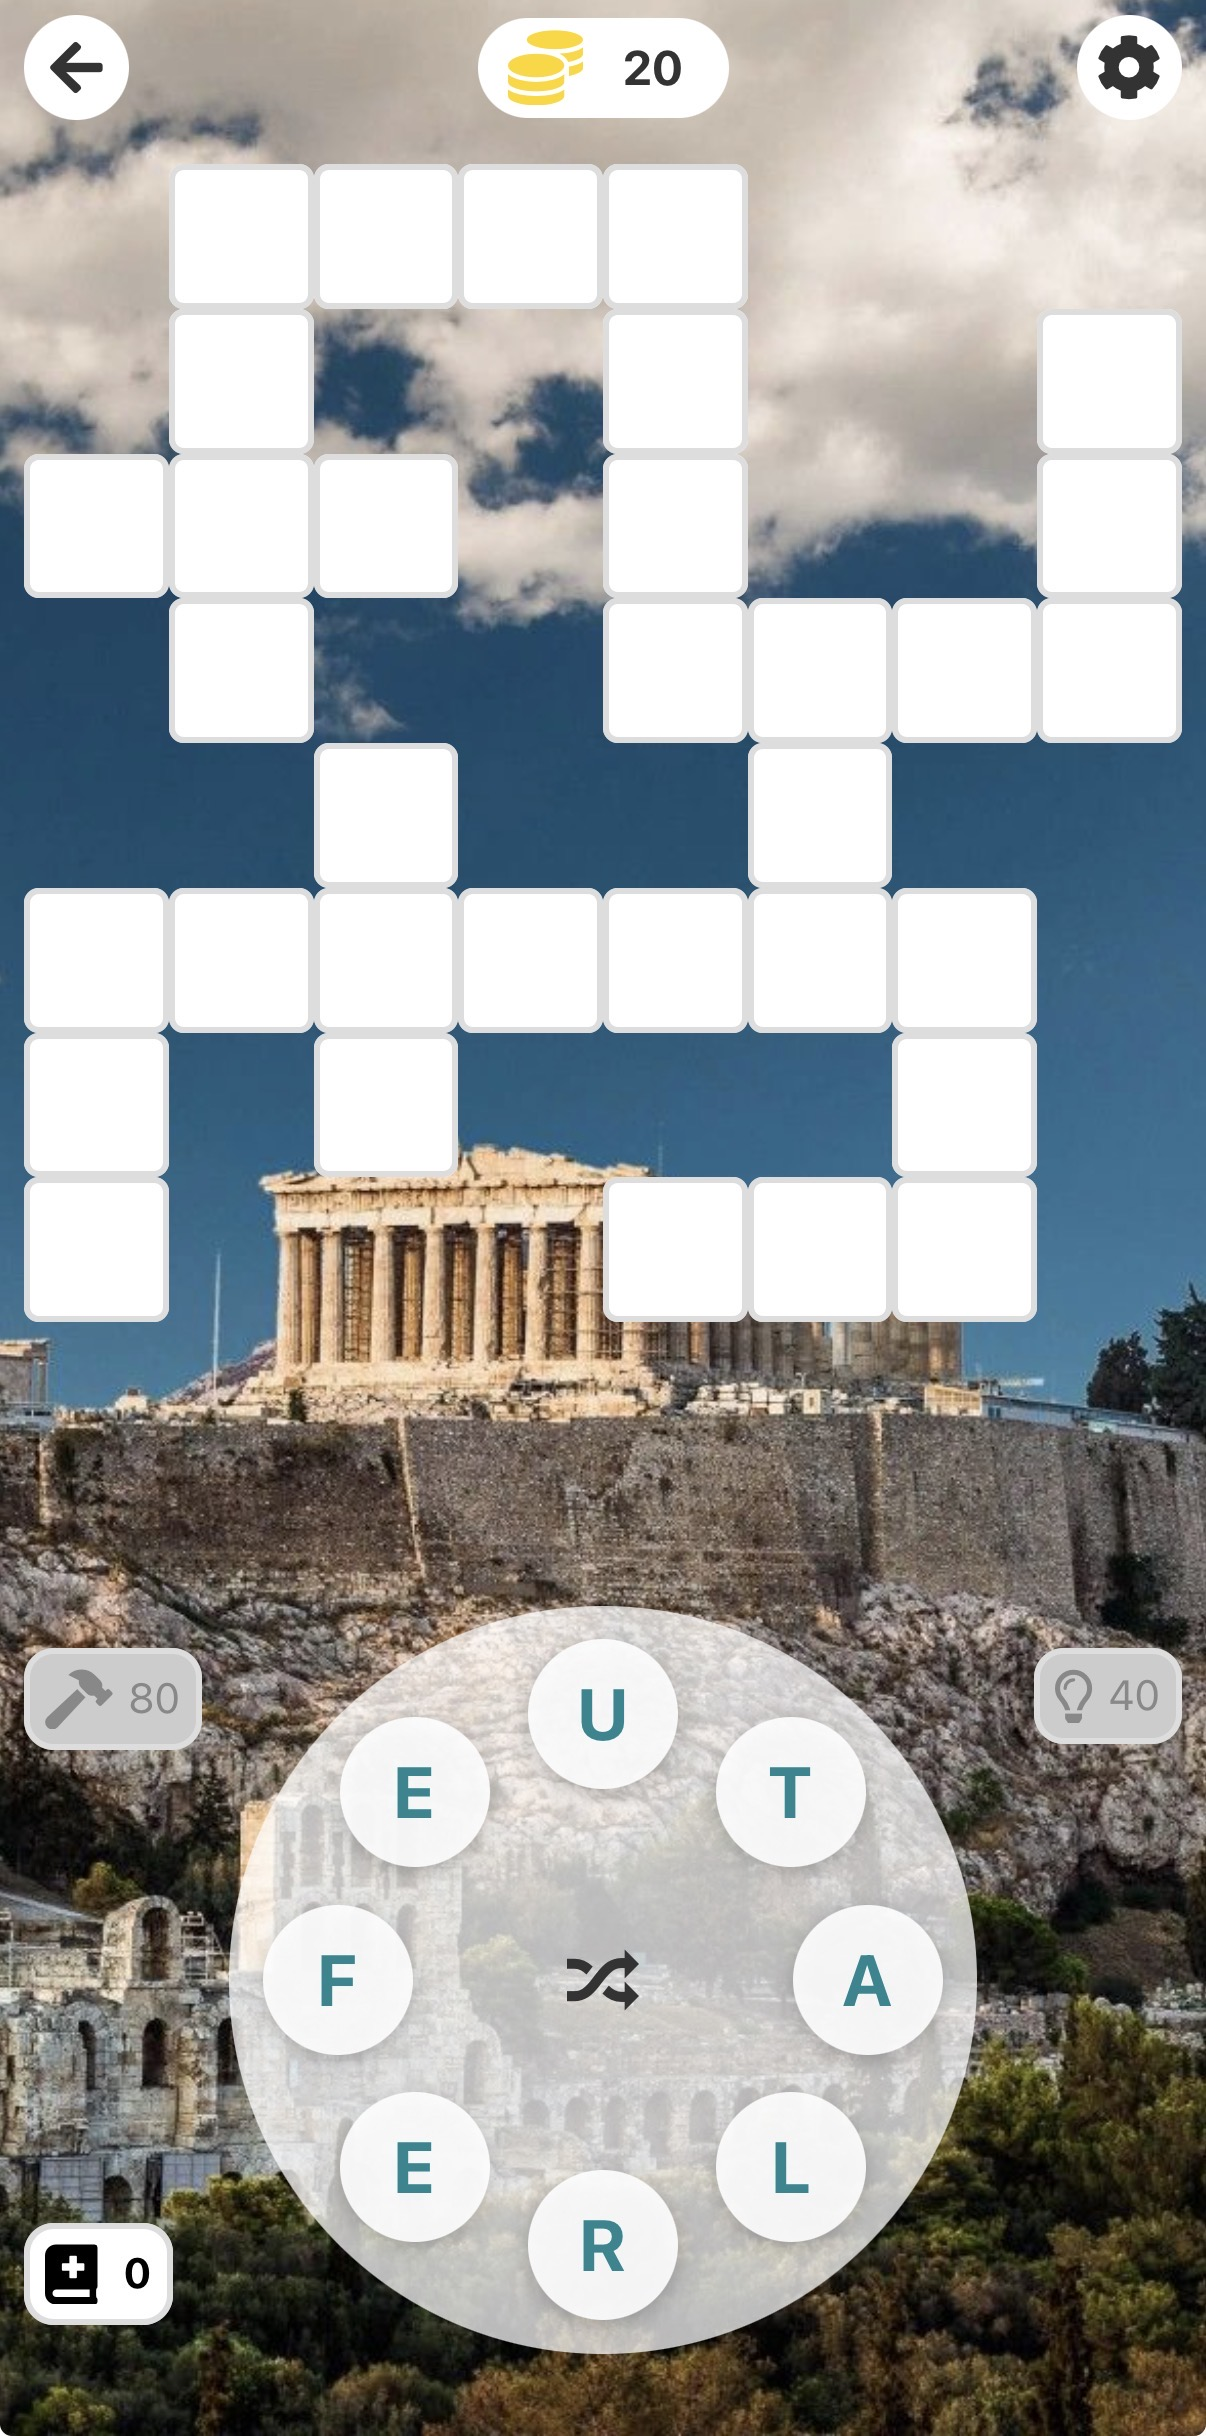
\includegraphics[width=\linewidth]{figures/wow_screenshot_b2.jpg}
            \caption{B2}
            \label{fig:wow_shot_b2}
        \end{subfigure}\hfill
        \begin{subfigure}[b]{0.31\textwidth}
            \centering
            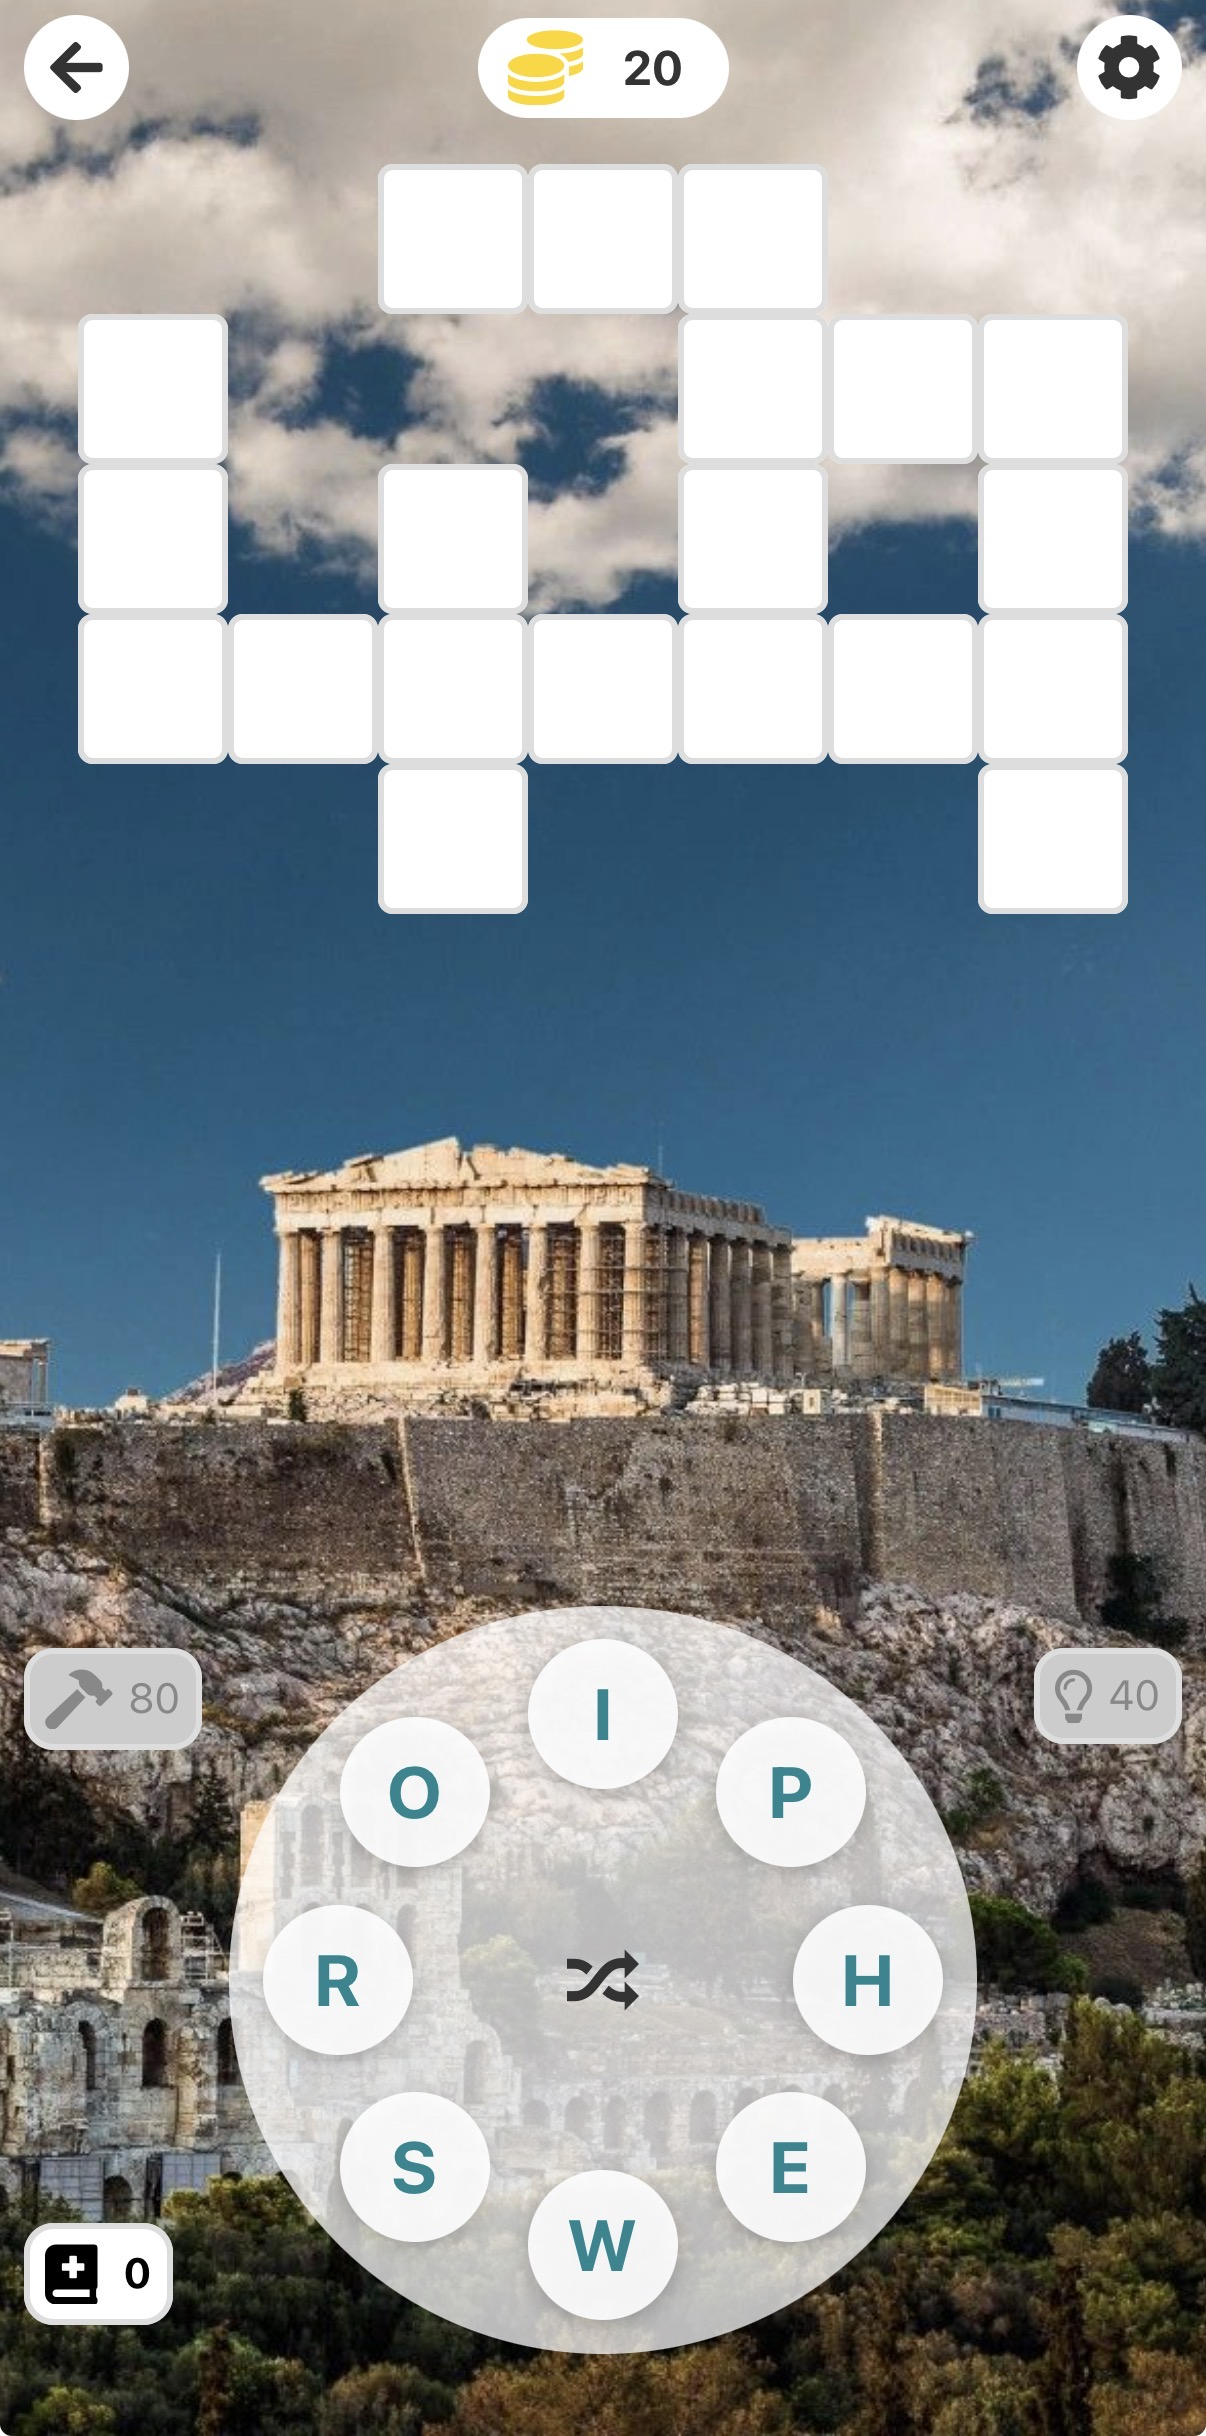
\includegraphics[width=\linewidth]{figures/wow_screenshot_c1.jpg}
            \caption{C1}
            \label{fig:wow_shot_c1}
        \end{subfigure}\hfill
        \begin{subfigure}[b]{0.31\textwidth}
            \centering
            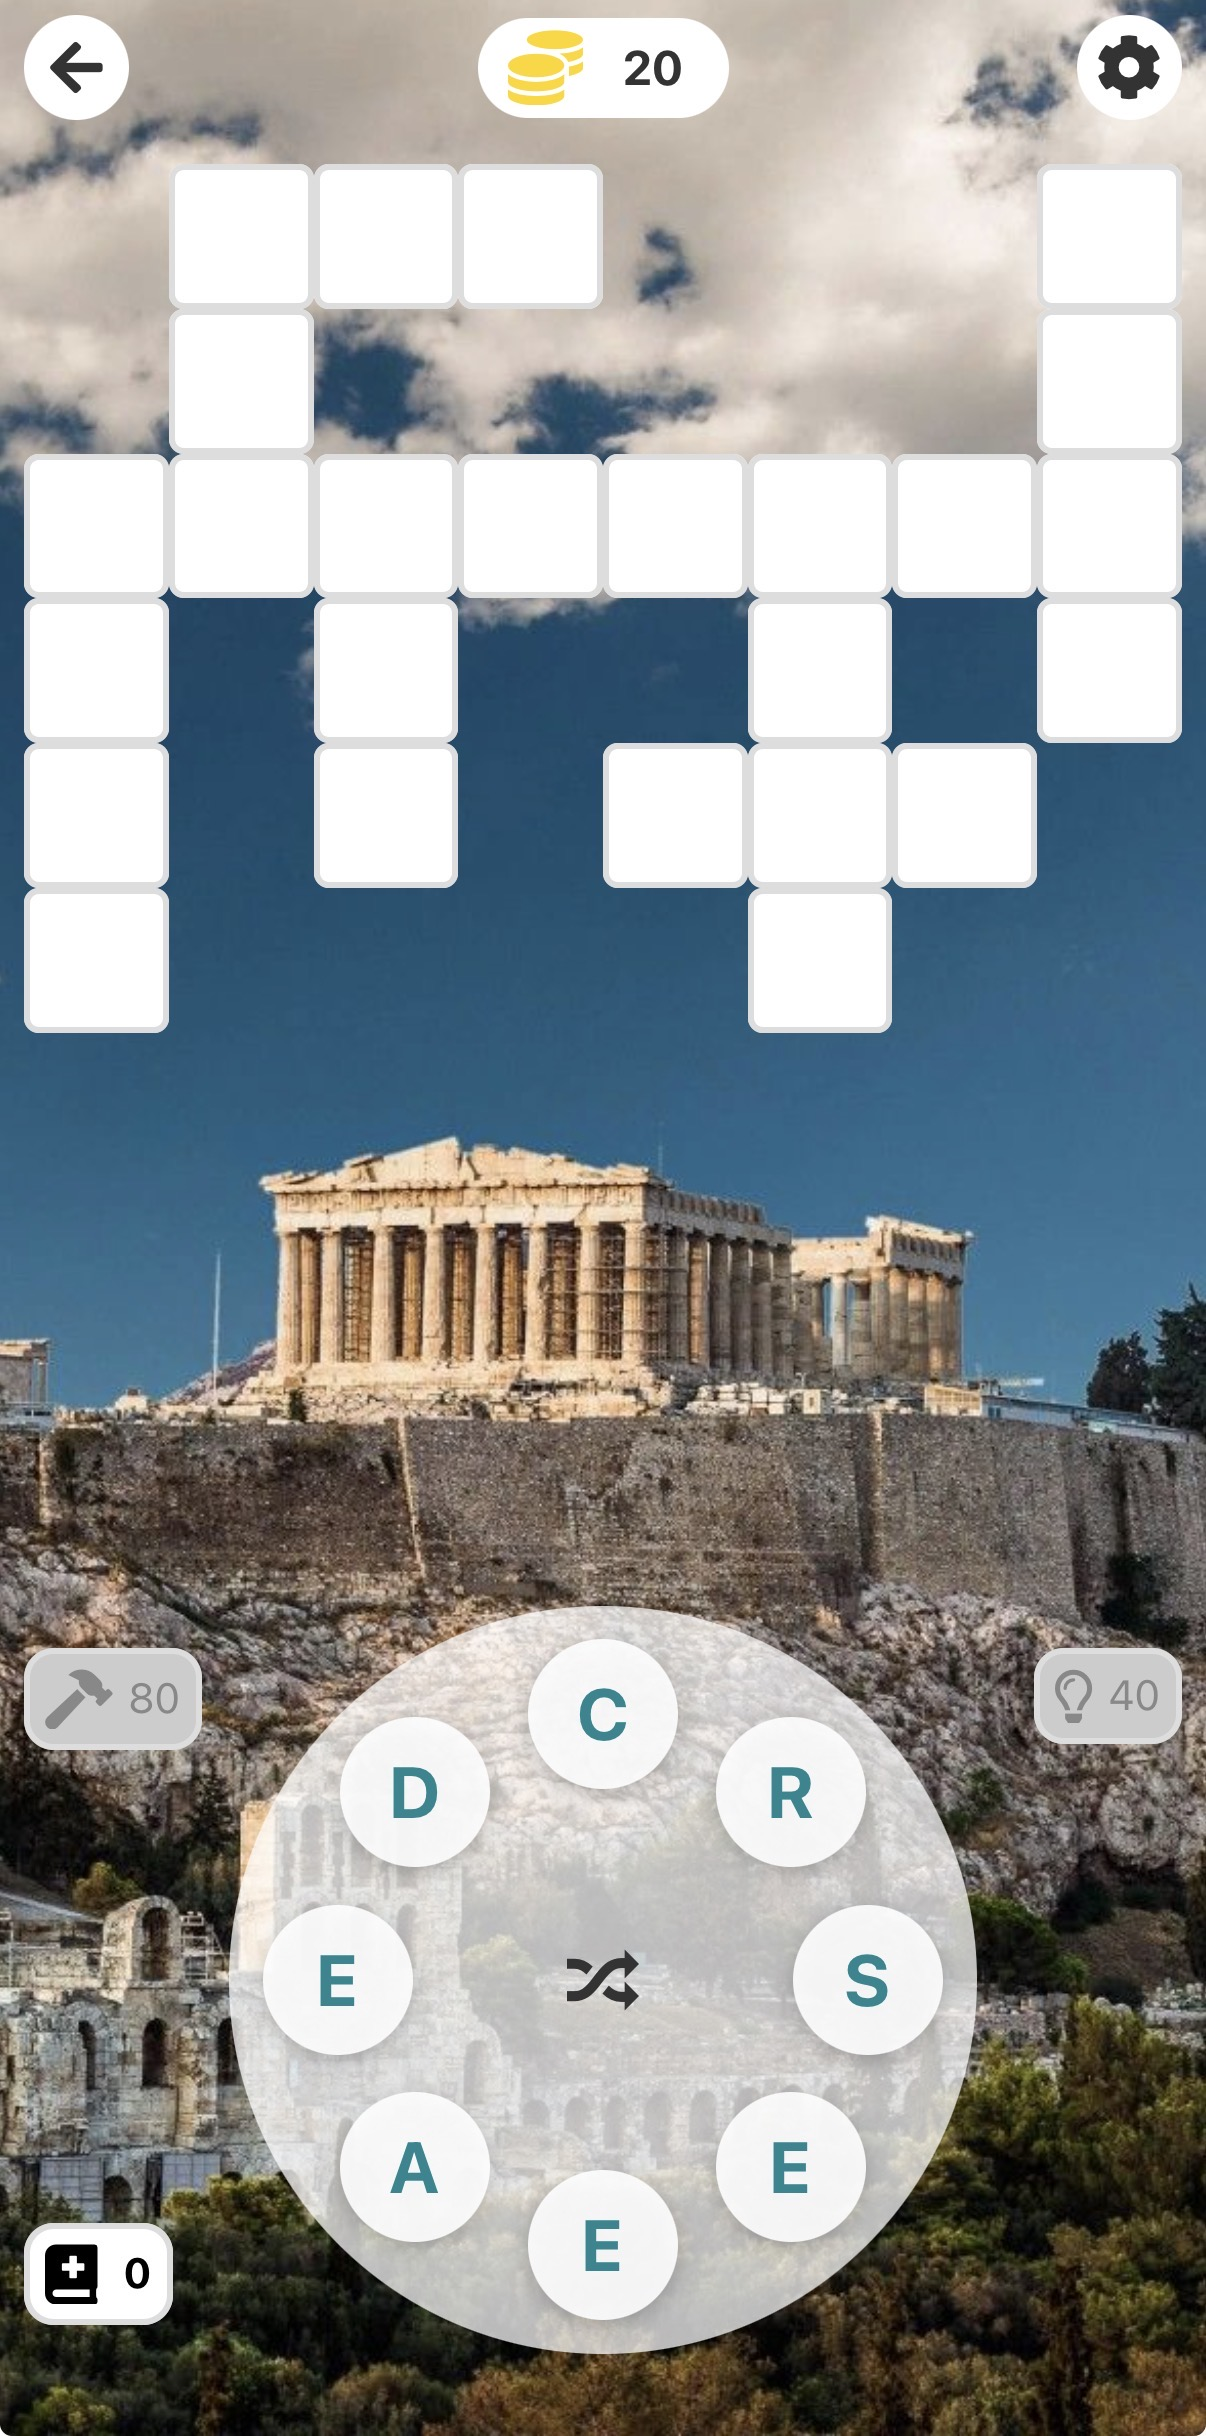
\includegraphics[width=\linewidth]{figures/wow_screenshot_c2.jpg}
            \caption{C2}
            \label{fig:wow_shot_c2}
        \end{subfigure}
        \caption{Word of Wonders boards generated on a physical device for an English learner who declared each of the six CEFR levels at onboarding, all other conditions held fixed. Board density visibly grows from a bare two-word cross at A1 to a multi-armed board of several intersecting words by B2--C2.}
        \label{fig:wow_screenshots_cefr}
    \end{figure}
    Figure~\ref{fig:wow_screenshots_cefr} shows the same generator running on a physical device, for one learner who selected each of the six CEFR levels in turn. The pattern corroborates Figure~\ref{fig:wow_words_placed} directly, but through a different mechanism than the benchmark's own uniform random sampling: proficiency-based vocabulary auto-seeding (Section~\ref{subsec:registration_impl}) inserts every word at every level \emph{below} the learner's declared one into \texttt{user\_vocabulary} at registration, so declaring A1 --- already the lowest level --- seeds nothing and leaves \texttt{GameLoader.js}'s \texttt{trackedWords} pool empty of anything beyond whatever the learner has reviewed since, while declaring C2 seeds the entire A1--C1 dictionary at once. The visibly sparse A1/A2 boards and the visibly denser B2--C2 ones are therefore a real instance of the same word-count effect Section~\ref{subsubsec:wow_eval_words_placed} measured synthetically, produced by the application's actual onboarding path rather than by the benchmark harness.

    \subsubsection{Generation Time}
    \label{subsubsec:wow_eval_gen_time}
    \begin{figure}[htbp]
        \centering
        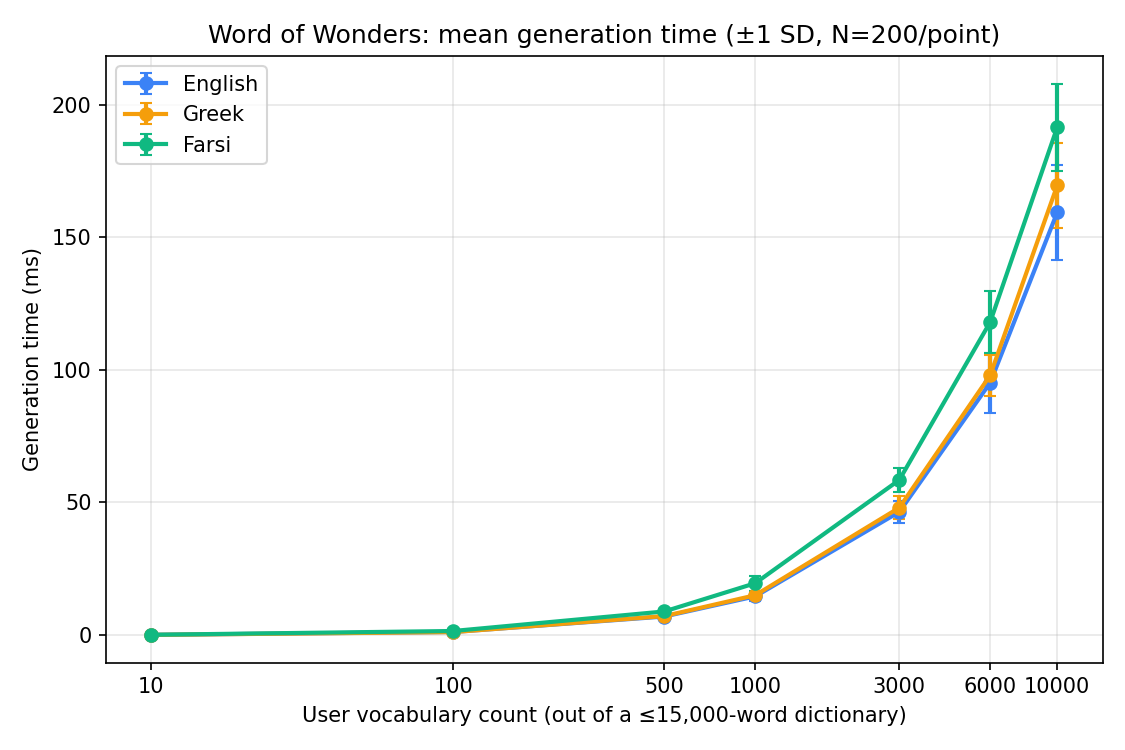
\includegraphics[width=0.8\textwidth]{figures/wow_generation_time.png}
        \caption{Mean grid-generation wall-clock time (ms) as a function of simulated tracked-vocabulary size, per language, measured under Node.js/V8 on a development machine. Error bars show $\pm 1$ standard deviation over 200 repetitions per point.}
        \label{fig:wow_generation_time}
    \end{figure}
    Figure~\ref{fig:wow_generation_time} shows generation time growing from sub-millisecond at a 10-word vocabulary to 159--192~ms at 10,000 words, with the three languages tracking each other closely throughout. The curve is visibly superlinear beyond roughly 3,000 words, consistent with \texttt{tryPlaceWord}'s per-candidate intersection search scaling with both the number of words already placed and the priority sort (Algorithm~\ref{alg:wow_priority}) running over the entire candidate pool on every call.

    These figures were measured under Node.js/V8 on a laptop, not under Hermes on an actual mobile device, and are reported here as evidence of the algorithm's \emph{scaling behaviour} --- no combinatorial blow-up and no failure at any tested scale --- rather than as a prediction of on-device latency: JIT and garbage-collection behaviour differ enough between V8 and Hermes, and between individual phones, that an absolute millisecond figure measured on one device would not transfer to another. \texttt{GameLoader.js} currently calls the generator synchronously on the JS thread (Section~\ref{subsec:wow_impl}), wrapped only in a zero-delay \texttt{setTimeout} to yield a render frame for the loading spinner, not to move the computation off-thread; the superlinear growth observed here means that a learner whose tracked vocabulary eventually reaches the thousands of words could, on slower hardware, experience a visibly longer wait than the benchmark's low-vocabulary numbers suggest. A direct mitigation, left as a concrete direction rather than spec here, is to move grid generation server-side --- the reels service's existing infrastructure (Section~\ref{sec:reels_service_impl}) already performs comparable per-request computation --- and push a precomputed board to the client opportunistically the next time it is online, trading a network round trip for a guaranteed, device-independent generation cost rather than an open question per phone.

    \subsection{Recommendation Engine: The Cold-Start Problem}
    \label{subsec:recommender_cold_start}
    Cold start --- a recommender system having little or nothing to personalise on for a given user --- is a well-known limitation of collaborative and content-based recommendation alike, not a defect specific to \textit{Glosy} \cite{adomavicius2005toward}. Section~\ref{subsec:cascade_hybrid} already gave this as the reason the engine has no collaborative-filtering stage at all: a cross-learner interaction matrix dense enough to be useful does not yet exist for a newly-launched application. What this section evaluates is how the same problem manifests one level down, inside Stage~3 itself, and what \textit{Glosy} currently does and does not do about it.

    Stage~3's profile vector (Section~\ref{subsec:stage3_design}) is built entirely from \texttt{reel\_interactions} --- the weighted sum of the TF-IDF vectors of reels a learner has liked, saved, shared, or commented on. Since every one of \textit{Glosy}'s current users is, by definition, a user who has not yet accumulated that history, \texttt{profile\_vector} is \texttt{None} for all of them today, and Section~\ref{subsec:cascade_design}'s graceful degradation takes over: the cascade's sort key collapses to (has-due-word, constant~0), i.e. Stage~2 plus a random tiebreak, with Stage~3 contributing nothing. This is not a rare edge case the design merely tolerates --- it is, at present, the actual ranking behaviour for the entire user base, for as long as no one has interacted with enough reels to build a profile from.

    \textit{Glosy} already has a partial, in-progress answer to this in its onboarding flow, one screen ahead of where the cascade could use it. The last onboarding page (\texttt{PersonalizationSlide.tsx}, Figure~\ref{fig:onboarding_personalization}) asks the learner to multi-select from a fixed set of eight topic chips --- Movies, Sports, Anime, Make up, Cartoons, Video games, News, Politics --- and to declare an age (16 upward, matching the declared Play Store audience), both required before onboarding can proceed. Both are persisted at registration: \texttt{preferences} as a comma-joined string and \texttt{age} as an integer, both columns on \texttt{users} (Section~\ref{sec:data_modelling}). Neither, however, is read anywhere in \texttt{reel\_service.py} --- not in Stage~3's profile construction, not anywhere else in \texttt{get\_personalized\_reels} or \texttt{get\_random\_reels}. The data is collected and stored; the recommendation engine simply does not look at it yet. This is a genuine gap rather than a documentation lag: the schema and the onboarding UI are already ahead of the recommendation code that would consume them.

    \begin{figure}[!htbp]
        \centering
        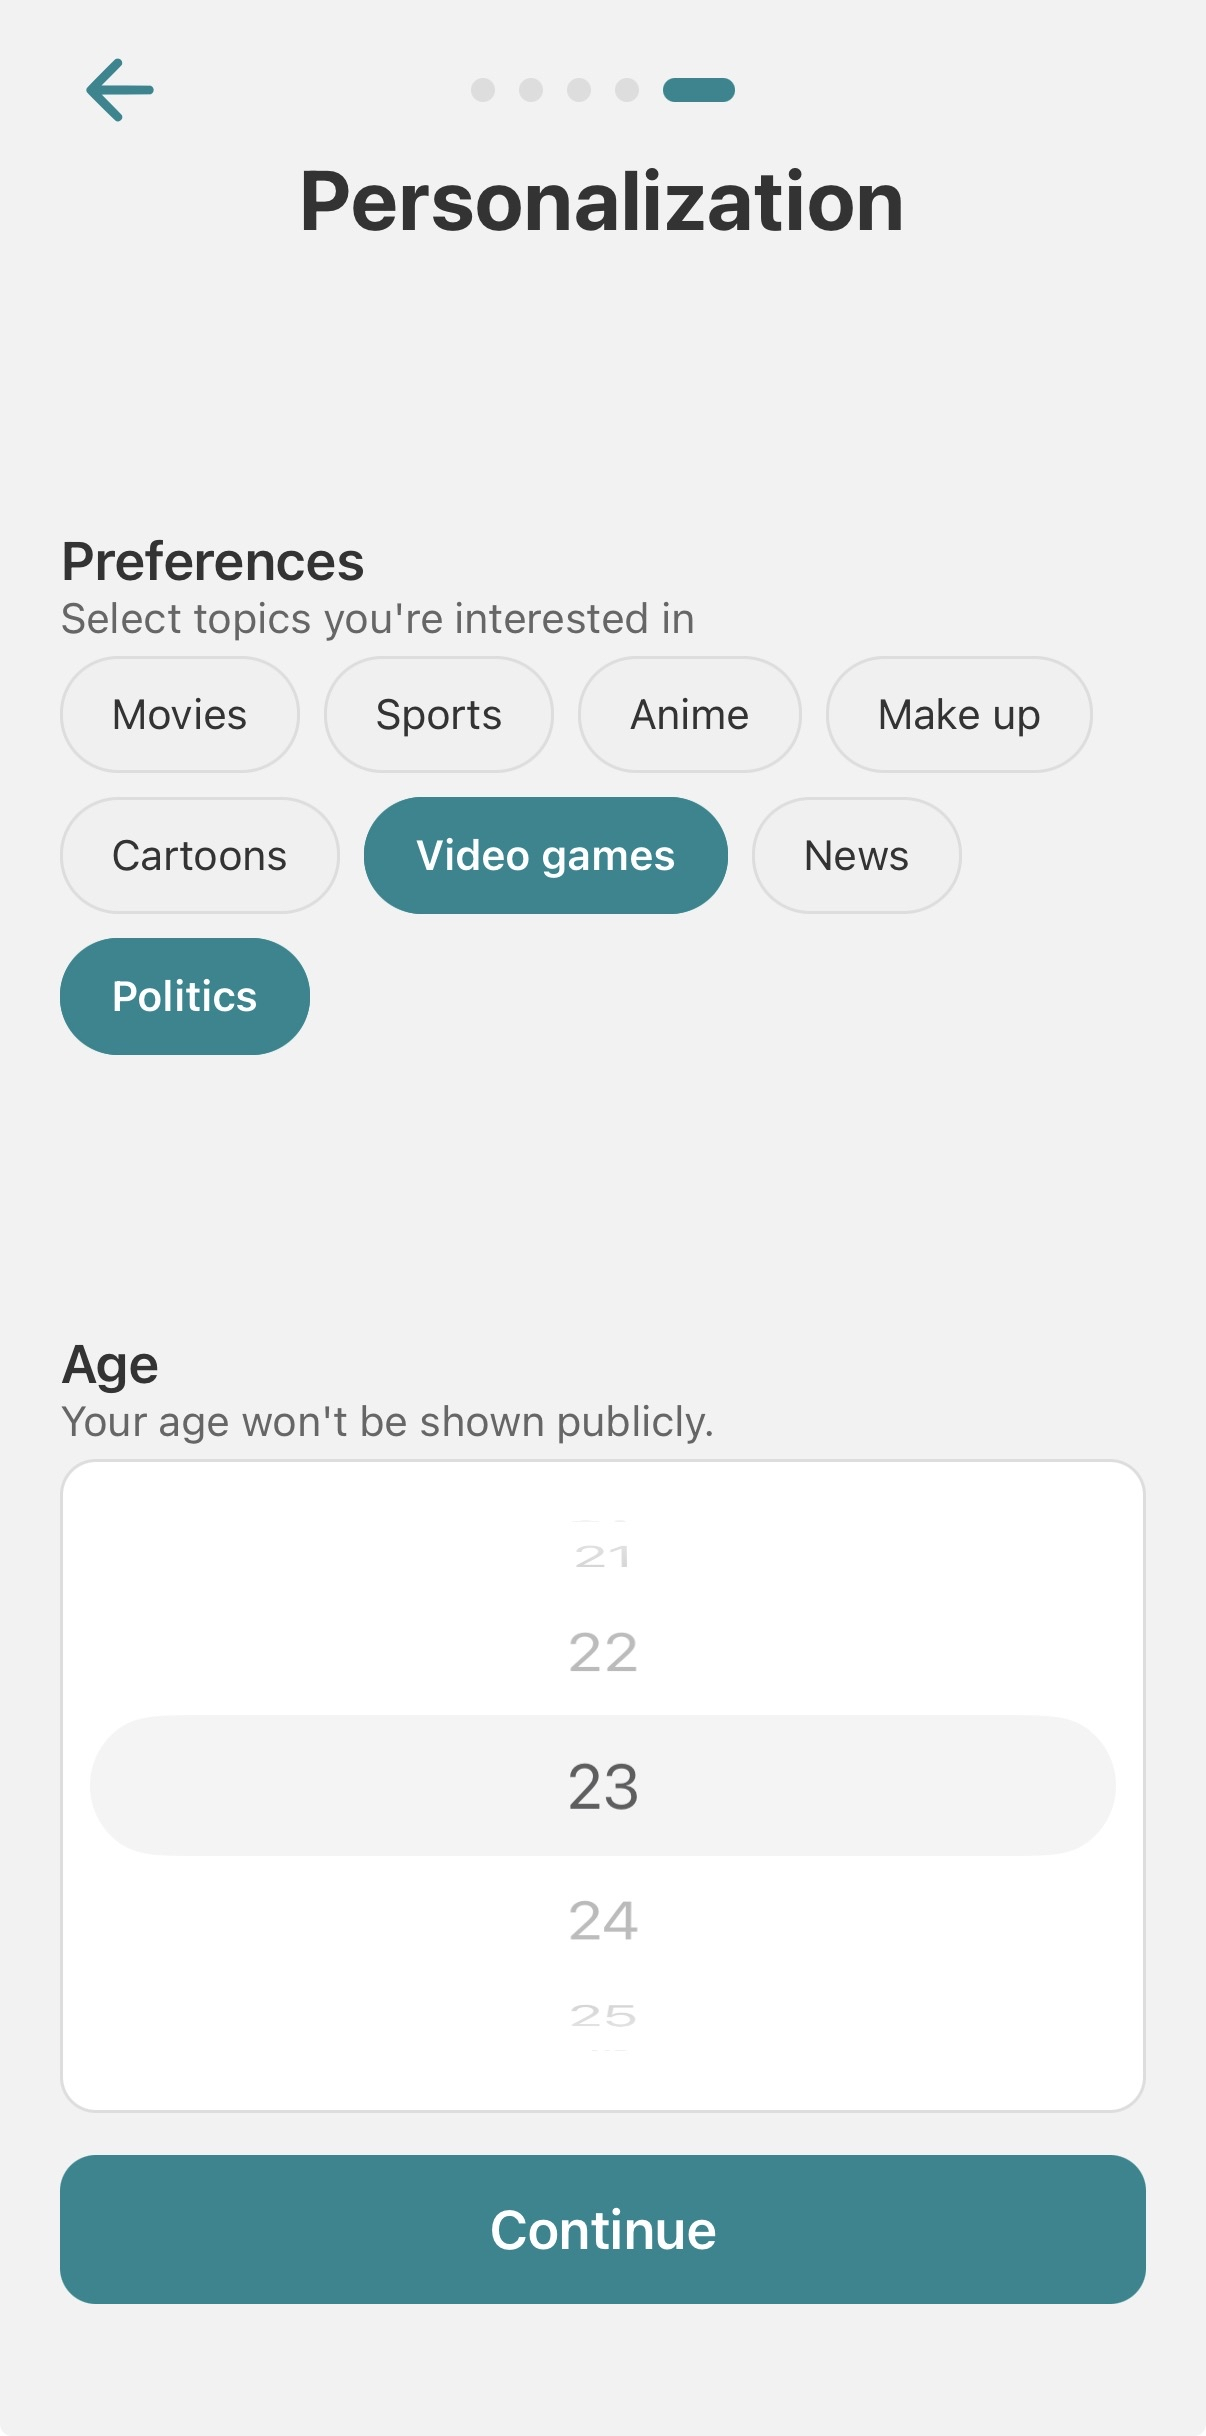
\includegraphics[width=0.28\textwidth]{figures/onboarding_personalization.jpeg}
        \caption{The Personalization screen (\texttt{PersonalizationSlide.tsx}), the last onboarding page}
        \label{fig:onboarding_personalization}
    \end{figure}

    Two concrete directions follow directly from this gap, both already anticipated by the existing structure rather than requiring a new data model: first, using the declared topic preferences as a cold-start substitute for Stage~3's profile vector --- a sensible prior for a learner who has stated an interest in, say, Sports, before they have liked a single reel, closing the gap identified in the paragraph above --- currently limited by the fixed, hand-picked eight-topic taxonomy the onboarding chips offer, with automated topic generation (deriving topics from reel content rather than a static hardcoded list) as the natural next step once a large enough content library makes that worth building; and second, age-conditioned recommendation, using the already-collected \texttt{age} column as a further ranking or filtering signal once a concrete policy for it is designed. Chapter~\ref{chapter:conclusions} is updated to carry both forward as named future-work items.

    \subsection{Recommendation Engine: Stage 1 Comprehensibility Filter}
    \label{subsec:stage1_eval}
    Stage~1's outcome (Section~\ref{subsec:stage1_design}) depends less on the filter itself than on the catalogue it is applied to: how many reels exist for the learner's language, how densely each reel's subtitles are tokenised (a reel with no tokenised word can never pass), and how many reels were recently recommended to the learner, since these are excluded for a 24-hour cooldown window. The results below are therefore illustrative rather than a property of the engine alone. The catalogue currently holds only 56 Farsi reels, inserted only to show how the filter behaves rather than curated as a learning library; 50 of the 56 have at least one tokenised word, and the other six can never pass yet.

    \begin{figure}[!htbp]
        \centering
        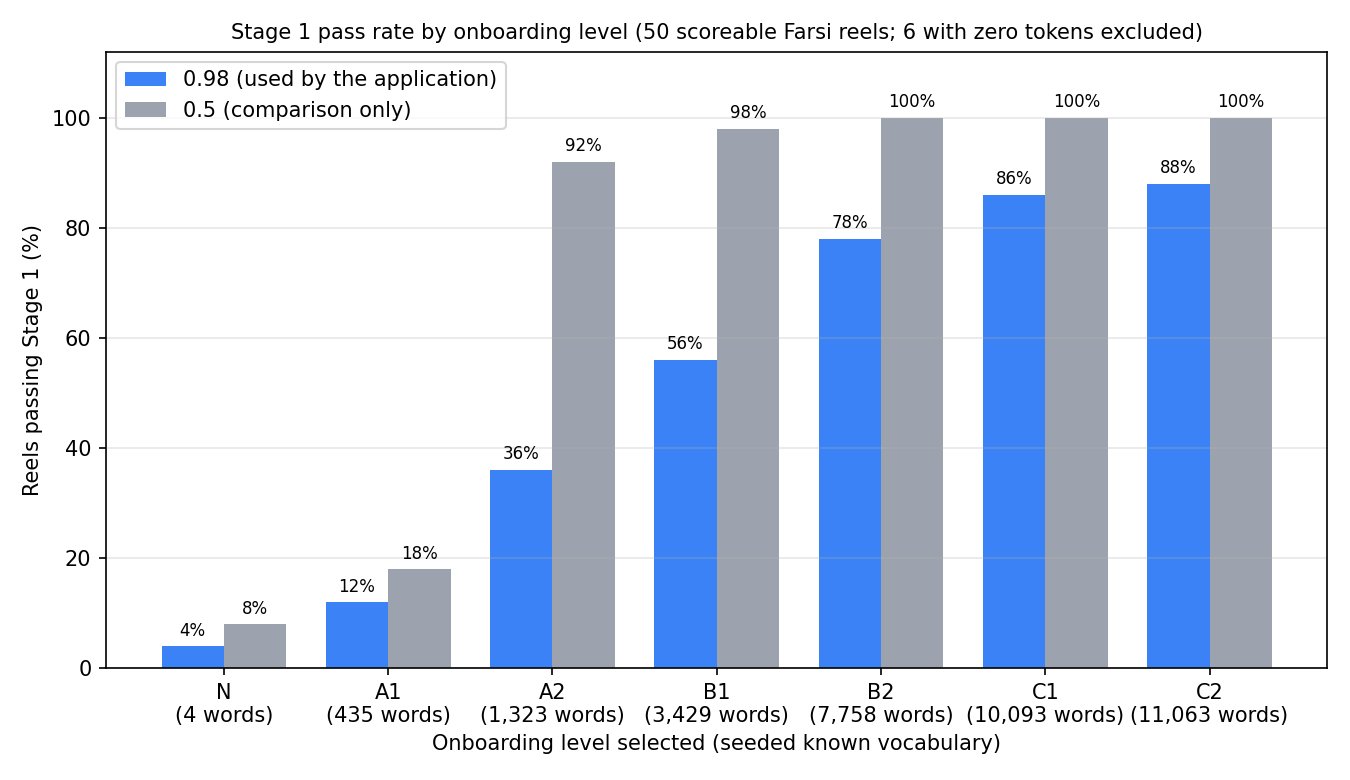
\includegraphics[width=0.80\textwidth]{figures/stage1_pass_rate.png}
        \caption{Share of the 50 tokenised Farsi reels passing Stage~1, per onboarding level, at the threshold the application uses (0.98) and, for comparison only, a looser one (0.5). Each level's known vocabulary is what registration seeds for it (Section~\ref{subsec:registration_impl}); level N receives only four starter words.}
        \label{fig:stage1_pass_rate}
    \end{figure}

    Figure~\ref{fig:stage1_pass_rate} shows that at the 0.98 threshold the application uses, beginners are barely served (level N: 4\%; A1: 12\%), the pass rate rises through A2 (36\%) and B1 (56\%), and it reaches only 88\% even at C2. For comparison, Stage~1 was also evaluated at a looser threshold of 0.5, which saturates from A2 upwards (92\%) but still passes only 8\% and 18\% of reels for levels N and A1. A looser filter therefore does not close the beginner gap: that needs easier content, not a lower threshold, and the application keeps the 0.98 threshold.

    \subsection{Recommendation Engine: Stage 2 Due-Word Prioritisation}
    \label{subsec:stage2_eval}
    Stage~2 (Section~\ref{subsec:stage2_design}) can only prioritise reels if the learner has words due for review. A learner who declares level N for Farsi has no lower level to seed vocabulary from, so onboarding instead adds four everyday starter words --- \textit{sal\={a}m} (hello), \textit{\={a}b} (water), \textit{b\={a}b\={a}} (dad) and \textit{ch\={a}y} (tea) --- as brand-new FSRS cards, all due immediately. The catalogue of 56 Farsi reels was assembled so that reels containing these words exist: 11 of the 56 contain at least one of them (\textit{sal\={a}m} in 5, each of the other three in 2).

    The scenario tested is a new user who has not registered and opens the reels feed. The frontend forwards the four due words with the request, and for a guest the server applies Stage~2 alone, since the comprehensibility filter and the content-based ranking both need an account. Running the reels service's own ranking and review-word assignment code on the real catalogue, over 2{,}000 repetitions, every reel on the first page of ten contains a due word, against 1.96 of ten for a page requested without due words, and all four words receive a review prompt on every page, each attached to a different reel. The mechanism therefore behaves as designed, but only because the catalogue was built around these four words: it holds just 11 such reels, so a second page can carry at most one more. As with Stage~1, what limits the feature is the size of the catalogue, not the ranking logic.

    \subsection{Recommendation Engine: Stage 3 Content-Based Ranking}
    \label{subsec:stage3_eval}
    Stage~3 (Section~\ref{subsec:stage3_design}) is not tested here. It is built entirely on scikit-learn's TF-IDF weighting and cosine similarity, an established library implementing a long-standing retrieval technique, so re-testing those components would evaluate the library rather than \textit{Glosy}. What remains specific to the system, its dependence on an interaction history that no user has yet accumulated, is discussed in Section~\ref{subsec:recommender_cold_start}.
 

\chapter{Conclusions \& Future work} \label{chapter:conclusions}
\section{Contributions}

\section{Limitations}
    The work presented in this thesis has several limitations that must be acknowledged honestly.
    % If no user tests
    \textbf{No empirical user study.} The pedagogical effectiveness of the system has not been evaluated in a controlled experiment.
    \textbf{Limited content library.} The current content library is limited in scope and diversity.

    \textbf{Steep onboarding barriers.} The Glosy same of LingQ, incorporates real-world texts, its interface poses steep onboarding barriers for novice learners \cite{karasimos2022battle}.

    \textbf{Lack of social scaffolding.} The system lacks mechanisms for social scaffolding through peer or native-speaker interaction.

    % Write this claude: some language are formal/informal spoken/written like farsi. English and Greek is not like that. Also some languages have suffixes and prefixes that form grammer like turkish and farsi. for example مادَر is mother and my mother in colloquial is مادَرَم. In English, we don't have that. that's why Tokenizers (hazm) fails to tokenize all words in farsi that are included in out database words table. In the future give option to manually tokenize words while creating a reel. 

\section{Future Work}
    The following directions are identified as high-value:
    \begin{sloppypar}
    \begin{itemize}
        \item \textbf{Automated content annotation pipeline:} A pipeline that ingests a raw video URL, transcribes speech using a large language model, aligns the transcript to video timestamps, tokenises and POS-tags the output, maps tokens to the word database, and produces a fully annotated reel record—reducing the per-reel curation cost from hours to minutes.
        \item \textbf{Empirical evaluation:} A randomised controlled study measuring vocabulary gain, retention at one week and one month, and learner engagement metrics, comparing Glosy against a no-game control condition and against Duolingo.
        \item \textbf{Multi-language expansion:} The schema and service layer are language-agnostic (language is a foreign key throughout); adding a new language requires only content ingestion, not code changes.
        \item \textbf{Collaborative learning features:} Shared vocabulary challenges, leaderboards scoped to friend groups, and comment-driven vocabulary discussion on individual reels, supporting the social dimension of Vygotsky's theory.
        \item \textbf{Vocabulary synchronisation performance:} Replacing the serial per-word UPDATE loop in \texttt{syncController.js} with a bulk \texttt{INSERT ... ON CONFLICT DO UPDATE} statement to support large offline sessions without latency degradation.
        % use Cache like Redis
        \item \textbf{Cold-start mitigation via onboarding preferences:} Wiring the topic preferences and age already collected by onboarding's \texttt{PersonalizationSlide.tsx} (Section~\ref{subsec:recommender_cold_start}) into Stage~3 as a cold-start substitute for the interaction-based profile vector, replacing its current fixed, hand-picked eight-topic taxonomy with automated topic generation derived from reel content once the library is large enough to support it.
        \item \textbf{Age-conditioned recommendation:} Using the \texttt{age} column, already collected at onboarding but currently unread by the recommendation engine, as a further ranking or filtering signal once a concrete policy for it is designed.
    \end{itemize}
    \end{sloppypar}

    
\newpage

% ----------Back-matter----------
\backmatter

% Bibliography
\bibliographystyle{unsrt}
\addcontentsline{toc}{chapter}{Bibliography}
\bibliography{references} % Use references.bib

% Abbreviations
\chapter*{Abbreviations}
\markboth{Abbreviations}{Abbreviations} % same reason as the Glossary below
\addcontentsline{toc}{chapter}{Abbreviations}
\pagestyle{headings}
% Abbreviations
% Two-column layout via the \gl macro (styles/ioniostyle.sty), as specified
% in the guidelines. Keep entries in alphabetical order.

\gl
{AI}
{Artificial Intelligence}

\gl
{CLT}
{Cognitive Load Theory}

\gl
{FSRS}
{Free Spaced Repetition Scheduler}

\gl
{HLR}
{Half-Life Regression}

\gl
{L2}
{Second Language}

\gl
{MALL}
{Mobile-Assisted Language Learning}

\gl
{SLA}
{Second Language Acquisition}

\gl
{SRS}
{Spaced Repetition System}

\gl
{ZPD}
{Zone of Proximal Development}

% Add additional abbreviations used in your thesis
% Example:
% \gl
% {[ABBREVIATION]}
% {[Full Description]}


% Glossary
\chapter*{Glossary}
\markboth{Glossary}{Glossary} % \chapter* sets no running head, so the multi-page glossary would inherit "Bibliography"
\addcontentsline{toc}{chapter}{Glossary}
\pagestyle{headings}
% Glossary of Terms
% Two-column layout via the \gl macro (styles/ioniostyle.sty), as specified
% in the guidelines. Keep entries in alphabetical order.

\gl
{Algorithm}
{A sequence of instructions for solving a problem}

\gl
{Comprehensible Input}
{Language input a learner can understand despite containing some unknown elements, per Krashen's Input Hypothesis ($i+1$)}

\gl
{Forgetting Curve}
{The exponential decline of memory retention over time in the absence of reinforcement, first described by Ebbinghaus}

\gl
{Gamification}
{The addition of game-design elements (points, streaks, badges) to a non-game task, as distinct from game-based learning}

\gl
{Lexical Coverage}
{The proportion of word tokens in a text that a reader already knows; 98\% coverage is the established threshold for unassisted comprehension}

\gl
{Recommender System}
{An algorithm that ranks or filters candidate items for a user based on content features, collaborative behaviour, or both}

\gl
{Spaced Repetition}
{A learning technique that schedules review of an item at increasing intervals timed to precede predicted memory decay}

\gl
{Testing Effect}
{The finding that actively retrieving information from memory produces better long-term retention than passive re-study}

\gl
{Zone of Proximal Development}
{The gap between what a learner can do unaided and what they can do with appropriate scaffolding, per Vygotsky's sociocultural theory}

% Add additional terms used in your thesis
% Example:
% \gl
% {[Term]}
% {[Definition/Explanation]}


% Index -- disabled: the thesis has no \index{} entries, so it would print nothing and the
% TOC line would point at an empty page. Re-enable once index terms are added.
% \newpage
% \addcontentsline{toc}{chapter}{Index}
% \printindex

% Closing blank page (guidelines: final blank page)
\clearpage
\thispagestyle{empty}\mbox{}

\end{document}